\documentclass[en,msc,data]{cseuoi-thesis} % Μεταπτυχιακό με ειδίκευση στην Επιστήμη και Μηχανική Δεδομένων (στα Ελληνικά)

%graph theory package
\usepackage{tikz}
\usetikzlibrary{positioning}
\usetikzlibrary{shapes.geometric}

%additional packages
\usepackage{subcaption}
\usepackage{enumerate}


%Custom theorem types
\newtheorem{prop}{Proposition}[chapter]
\newtheorem{assumption}{Assumption}[chapter]

% 
% Συμπληρώστε τα στοιχεία σας στις παρακάτω εντολές (αφαιρώντας το \colorbox{gray}{})
%
\titleGr{{Detection of Fake News in Tree Propagation Networks}}
\titleEn{{Detection of Fake News in Tree Propagation Networks}}
\authorGr{{Γεωργιάδης Ιωάννης}}
\authorEn{Georgiadis Ioannis}
\arthro{{τον}}
\aitiatiki{{Γεωργιάδη Ιωάννη}}
\dateGr{{Αύγουστος 2021}}
\dateEn{{August 2021}}
\advisorGr{{Σπυρίδων Κοντογιάννης, Αναπληρωτής Καθηγητής}}
\advisorEn{{Spyridon Kontogiannis, Associate Professor}}

%Epitropi
\MSCexaminer{Spyridon Kontogiannis}{Assoc.\ Professor}%
    {Department of Computer Science and Engineering, University of Ioannina (Advisor)}
\MSCexaminer{Loukas Georgiadis}{Assoc.\ Professor}%
    {Department of Computer Science and Engineering, University of Ioannina}
\MSCexaminer{Christos Nomikos}{Assist.\ Professor}%
    {Department of Computer Science and Engineering, University of Ioannina}


% Πακέτο για την εμφάνιση περιθωρίων (χρήσιμο για την εύρεση overfull boxes)
%\usepackage{showframe}

% Πακέτο για τη διατήρηση των floats (εικόνες κ.α.) εντός των ενοτήτων
\usepackage[section]{placeins}

% AE: Πακέτο για grid
%\usepackage[grid, texcoord, gridunit=pt, gridcolor=blue!40, subgridcolor=blue!20]{eso-pic}

\begin{document}

% Σελίδες χωρίς αρίθμηση
\pagenumbering{gobble}

% Εκτύπωση της σελίδας τίτλου
\maketitle

% Εκτύπωση της σελίδας με τις επιτροπές
\makecommittees

% Αρχικοποίηση του minitoc
\dominitoc[n]

\chapter*{\cseafierwsi}

To my family.

\bigskip

 % Προαιρετικό
\chapter*{\cseeuxaristies}

I would like thank and express my gratitude to my supervisor, Prof. Spyridon Kontogiannis for his guidance and support throughout my research. I would also like to thank those who supported me all those years, especially my family.

\bigskip

 % Προαιρετικό


% Σελίδες με αρίθμηση i, ii, iii, iv, ...
\pagenumbering{roman}

% Περιεχόμενα
\pdfbookmark{\contentsname}{contents} % hyperref
\tableofcontents

% Κατάλογος Σχημάτων
\addstarredchapterc{\listfigurename} % minitoc
\listoffigures

% Κατάλογος Πινάκων
\addstarredchapterc{\listtablename} % minitoc
\listoftables

% Κατάλογος Αλγορίθμων
\addstarredchapterc{\listalgorithmname} % minitoc
\listof{algorithm}{\listalgorithmname}

%\chapter*{\glossaryname}
% Εισαγωγή του κεφάλαιου στα περιεχόμενα
\addstarredchapter{\glossaryname} %minitoc

Η σελίδα αυτή είναι προαιρετική.
Περιέχει ορισμούς και επεξηγήσεις εννοιών, όρων, συντομεύσεων, και συμβολισμών.
Αν η έκτασή τους είναι μεγαλύτερη από δύο σελίδες τότε πρέπει να πάει στο τέλος της διατριβής, αμέσως μετά τα παραρτήματα. % Προαιρετικό

% Περίληψη και εκτεταμένη περίληψη
\chapter*{\abstractname}
\addstarredchapter{\abstractname} % minitoc
\makecseabstract

The proliferation of fake news in online social media platforms has opened up novel, multidisciplinary directions of research trying to achieve automated mechanisms for the timely identification and containment of fake news, and mitigation of its widespread impact on public opinion. While much of the earlier research was focused on identification of fake news based on its contents (e.g., writing style of the story, stance of involved reactions to it, linguistic analysis, etc.), or on the related context (e.g., exploitation of users’ engagement and their reputation within the social media platform, etc.), which are mostly based on AI-enabled techniques, there has been a rising interest in the provision of proactive intervention strategies which are mostly based on the analysis of the spatio-temporal characteristics of the evolving story within the underlying propagation network infrastructure. Most of these works mainly focus on the analysis of the time-series of the reactions to the stories. Some recent works focus on the structural characteristics of the propagation network. For example, it has been experimentally observed that a typical fake-news story evolves faster, deeper and farther than a typical true-story, within the social network platform.


In this thesis we continue the line of research focusing on the structural characteristics of the underlying propagation network. Our first differentiation from the literature is that we adopt a probabilistic model for the creation of stories, in which each story is created either by an expert (and is perceived as a \emph{true story}, or by some propagandist (and is then perceived as a \emph{fake story}). Experts have a high probability of providing the correct answer to the question posed by the story, e.g., because they are based on concrete arguments and scientific evidence. Propagandists, on the other hand, simply try to promote a particular stance (in favor of, or against the ground-truth answer) with the story, irrespective of the ground-truth. It should be noted that both an expert and a propagandist might provide either a correct or a false answer, but the expert is highly likely to be correct.


The above mentioned probabilistic model was proposed by Papanatasiou (2019), and was then studied and analyzed for a very simplified case in which the underlying propagation network is a simple directed path. In this thesis we provide a similar analysis for the case in which the underlying propagation network is a rooted directed tree. This is a much more challenging case, since the sequential nature of the users' reactions to an emergent story (and the direct consequences of their own actions to the entire story) no longer holds.


We first provide a careful analysis of the users' behavior during the evolution of the story, assuming that they behave rationally, i.e., they are expected-utility maximizers based on their own prior and posterior beliefs for the ground-truth value and for the type (true/fake) of the story. We then proceed with the involvement also of the platform, as an independent observer of the entire propagation network. Our goal is to determine an efficient mechanisms for the platform in order to decide in real-time whether and when exactly to intervene the evolution of an emerging story, while only observing in the underlying propagation tree.  

\noindent 

\bigskip


\chapter*{\cseextabstract}
\addstarredchapter{\cseextabstract} % minitoc
\makecseextabstract

Το φαινόμενο των ψευδών ειδήσεων στις διαδικτυακές πλατφόρμες κοινωνικής δικτύωσης έχει δημιουργήσει διεπιστημονικές κατευθύνσεις έρευνας που προσπαθούν να επιτύχουν αυτοματοποιημένους μηχανισμούς για τον έγκαιρο εντοπισμό και περιορισμό των ψευδών ειδήσεων όπως και την αποτροπη εκτεταμένων επιπτώσεών τους στην κοινή γνώμη. Ενώ ένα μεγάλο μέρος της προηγούμενης έρευνας επικεντρώθηκε στον εντοπισμό ψευδών ειδήσεων με βάση το περιεχόμενό τους, το οποιο εκμεταλευετε χαρακτηριστικα οπως το ύφος γραφής της ιστορίας, τη στάση των εμπλεκόμενων αντιδράσεων σε αυτήν, τη γλωσσική ανάλυση. Επισης, υπαρχουν προσσεγγισεις οι οποιες εξεταζουν το σχετικό πλαίσιο οπως η εκμετάλλευση της εμπλοκής των χρηστών και της φήμης τους εντός της πλατφόρμας κοινωνικής δικτύωσης. Πολλες απο τις παραπανω τεχνικες βασίζονται κυρίως σε τεχνικές με δυνατότητα τεχνητής νοημοσύνης οι οποιες παρουσιαζουν καποια μειονεκτηματα οσον αφορα την λυση που παρεχουν στο ζητημα τον ψευδων ειδησεων. Μια αλλη ενδιαφερουσα προσεγγιση για την παροχή στρατηγικών προληπτικής παρέμβασης, ειναι τεχνικες οι οποίες βασίζονται κυρίως στην ανάλυση των χωροχρονικών χαρακτηριστικών της εξελισσόμενης ιστορίας εντός της υποκείμενης υποδομής δικτύου διάδοσης. Οι περισσότερες από αυτές τις εργασίες επικεντρώνονται κυρίως στην ανάλυση των χρονοσειρών των αντιδράσεων στις ιστορίες. Ορισμένες πρόσφατες εργασίες επικεντρώνονται στα δομικά χαρακτηριστικά του δικτύου διάδοσης. Για παράδειγμα, έχει παρατηρηθεί πειραματικά ότι μια τυπική ψευδή είδηση εξελίσσεται ταχύτερα, βαθύτερα και μακρύτερα από μια τυπική αληθινή ιστορία, εντός της πλατφόρμας του κοινωνικού δικτύου.


Στην παρούσα διατριβή συνεχίζουμε τη γραμμή της έρευνας που επικεντρώνεται στα δομικά χαρακτηριστικά του υποκείμενου δικτύου διάδοσης, το οποίο προκύπτει από τις υποθέσεις εργασίας που εισάγουμε για την συμπεριφορά των χρηστών. Η πρώτη μας διαφοροποίηση από τη βιβλιογραφία είναι ότι υιοθετούμε ένα πιθανοθεωριτικό μοντέλο για τη δημιουργία ιστοριών, στο οποίο κάθε ιστορία δημιουργείται είτε από έναν ειδικό και γίνεται αντιληπτή ως \emph{αληθής ιστορία}, είτε από κάποιον προπαγανδιστή και στη συνέχεια γίνεται αντιληπτή ως \emph{ψευδή ιστορία}. Οι ειδικοί έχουν μεγάλη πιθανότητα να δώσουν τη σωστή απάντηση στο ερώτημα που θέτει η ιστορία, επειδή για παράδειγμα βασίζονται σε συγκεκριμένα επιχειρήματα και επιστημονικά στοιχεία. Οι προπαγανδιστές, από την άλλη πλευρά, απλώς προσπαθούν να προωθήσουν μια συγκεκριμένη στάση, υπέρ ή κατά ενός πραγματικού γεγονότος με την ιστορία, ανεξαρτήτως της πραγματικής αλήθειας. Θα πρέπει να σημειωθεί ότι τόσο ένας εμπειρογνώμονας όσο και ένας προπαγανδιστής μπορεί να δώσουν είτε μια σωστή είτε μια λανθασμένη απάντηση, αλλά ο εμπειρογνώμονας είναι πολύ πιθανό να είναι σωστός.


Για το προαναφερθέν πιθανοθεωριτικό μοντέλο υπάρχει ήδη μια ανάλυση για μια πολύ απλοποιημένη περίπτωση στην οποία το υποκείμενο δίκτυο διάδοσης είναι ένα απλό κατευθυνόμενο μονοπάτι. Στην παρούσα διατριβή παρέχουμε μια παρόμοια ανάλυση για την περίπτωση στην οποία το υποκείμενο δίκτυο διάδοσης είναι ένα ριζωμένο κατευθυνόμενο δέντρο. Η μετάβαση από την απλούστερη περίπτωση στην περίπτωση των δενδρικών δικτύων, αποτελεί πρόκληση καθώς δεν ισχύει πλέον η διαδοχική φύση των αντιδράσεων των χρηστών σε μια αναδυόμενη ιστορία και οι άμεσες συνέπειες των δικών τους ενεργειών σε ολόκληρη την ιστορία. Ένα σημαντικό χαρακτηριστικό του μοντέλου, το οποίο θεωρούμε ότι προσεγγίζει το γενικότερο πρόβλημα καλύτερα από άλλες εργασίες, είναι το γεγονός ότι λαμβάνετε υπ' όψιν κάποιου είδους οικονομικών παραγόντων κατά την εξέλιξη του φαινόμενου.


Αρχικά παρέχουμε μια προσεκτική ανάλυση της συμπεριφοράς των χρηστών κατά την εξέλιξη της ιστορίας, υποθέτοντας ότι συμπεριφέρονται ορθολογικά, δηλαδή επιδιώκουν την μεγιστοποίηση της αναμενόμενης ωφέλειας με βάση τις δικές τους προηγούμενες και μεταγενέστερες πεποιθήσεις για την τιμή της βασικής αλήθειας και για τον τύπο της ιστορίας (αληθής ή ψευδής). Με βάση τις υποθέσεις εργασίας που εισάγουμε για τους χρήστες, παραθέτουμε κάποιες παρατηρήσεις για την εξέλιξη της διαδικασίας μετάδοσης μιας είδησης σε ένα τέτοιο δίκτυο Στη συνέχεια, προχωρούμε με τη συμμετοχή και της πλατφόρμας, ως ανεξάρτητου παρατηρητή ολόκληρου του δικτύου διάδοσης. Στόχος μας είναι να καθορίσουμε έναν αποτελεσματικό μηχανισμό για την πλατφόρμα, ώστε να αποφασίζει σε πραγματικό χρόνο αν και πότε ακριβώς θα παρέμβει στην εξέλιξη μιας αναδυόμενης ιστορίας, παρατηρώντας μόνο στο υποκείμενο δέντρο διάδοσης. Τέλος, παραθέτουμε φραγματικές τιμές για την αναμενόμενη ωφέλεια της πλατφόρμας για την προσέγγιση του εντοπισμού του βέλτιστου χρόνου παρέμβασης.



\noindent 

\bigskip




% Σελίδες με αρίθμηση 1, 2, 3, 4, ...
\pagenumbering{arabic}

% Εισαγωγή των κεφαλαίων
%
% --- MAIN CONTENT ---
\chapter{Introduction}
\label{ch:Introduction}


\section{Motivation}
\label{sec:Motivation}
Social media has become an important part of our daily interactions due to its easy accessibility for users. According to \footnote{\url{https://datareportal.com/reports/digital-2021-april-global-statshot}} the user base of social media such as Facebook, YouTube, Twitter and Reddit is doubled since 2015. Hence, social media has become a massive hub for information sharing and many users choose to consume news from social media platform such the above mentioned. This ease of access to social media platforms accompanied with the ability to publish information in form of news article, which is given to regular users as well, creates the phenomenon of misinformation spreading. Most recent important cases of fake news, that brought spotlight to this problem, are the U.S. presidential elections of 2016 \footnote{\url{https://news.stanford.edu/2017/01/18/stanford-study-examines-fake-news-2016-presidential-election/}} and similar incidents in Germany's election of 2017\footnote{\url{https://www.theguardian.com/world/2017/jan/09/}}. 

Researches on fake news and rumor propagation attract the academic community. There is a collection of surveys that provide an overview of the problem, techniques and challenges, such as ~\cite{Zubiaga_2018,sharma2019combating,TrueFalseNewsOnline}. Approaches on fake news detection and mitigation might vary, but there are two core concepts that are common. First, there should be a way to describe and formulate human interactions and how they share information in their ecosystem, such as a social media platform. The second core concept is based on the above formulation, that describes those interactions. Based on these formulas, an approach should devise efficient methods that detect, mitigate or even prevent the spread of rumors and fake news.

There are many interesting challenges related to the topic of fake news and rumor propagation. First and foremost, the human nature that is hard to describe or formulate for a system to process it. Understanding human behavior on the topic of fake news is important in order to improve algorithms or other ways of automation in order to prevent this phenomenon. There is a plethora of researches, similar to ~\cite{FAKEnewsCovidERA,TrueFalseNewsOnline,ImpliedTEpennycock} that provide us with hints and information in order to understand human behavior on fake news detection. A second challenge is the motive behind the spread of misinformation. The reasons might be financial, political or even based on satire. This challenge is similar to that which concerns human behavior but we specify this explicitly because the development of such model rely heavily on those motives. Such an example is YouTube where users acquire advertisement revenue based on number of views. An attractive video that contains rumors, or misinformation in general, increases the income that it generates. The fact that more users have access to social media platforms creates another issue, that is the classification of rumors. The amount of posts shared within those networks is hard to monitor and classify in order to be used for training in machine learning models. Many platforms rely on fact checking from professional journalist, that specialize on this domain. 

On the topic of fake news detection, there are several techniques from different perspectives that deal with the phenomenon of fake news detection and mitigation. One of the most common models used to deal with fake news is the epidemic model. Epidemics tend to describe precisely the propagation of fake news inside social networks because of the similarities they have concerning structure of such networks as well the propagation dynamics. Some notable researches that refine and adjust the basic epidemic models presented in ~\cite{Kleinberg}, are ~\cite{SEIZ,SIHR_probGeneratingFunct,EpidemicMeanField,SimpleSIHR,VirusWithProfiles,NetworkTopologyEpidemics}. The drawback with epidemics is that they are time inefficient since they depend on observing the rates at which the population transition occurs between different states. Aside from propagation analysis, there are linguistics-based techniques that use the content of the information in order to detect fake news. Those approaches can be effective in some cases but they suffer from the fact that most of the time we do not have the exact values of ground truth in order to train those models ~\footnote{Models that do linguistic analysis are leveraging machine learning models.}. 


\section{Objectives}
\label{sec:Objectives}
Propagation analysis seems prominent approach in order to solve the problem of detecting fake news in online social media platforms. An interesting model is provided in ~\cite{papanastasiou} which is a sequential model that consists of a network of agents and a platform that monitors behaviors in that network ~\footnote{We provide every detail that we use from ~\cite{papanastasiou} but we strongly suggest the reader to study for deeper insight.}. Although social networks in real applications are by far more complex, the philosophy of this sequential model can be extended to more complex case studies. Our main objective in this thesis is to improve and adjust this model in order to work for tree propagation networks which is more representative version of a real world scenario and mitigate the problem faster than the approaches in related literature.

This modification comes with challenges concerning complexity of calculations that arise from the fact that social networks are complex structures. For this challenge, we assume in this thesis that the network we are working on is an $m$-ary tree, which is a more realistic representation of a social structure than the sequential model based on paths provide. This transition form a simple path to an $m$-ary tree comes with challenges such the formulation of propagation dynamics and the complexity of calculations from platform's side. We deal with this issue by providing the appropriate assumptions. First and foremost, we assume that platform, which can be seen as an \textit{super} agent, possess some distributional information about the other agents' prior beliefs of the story's type (true or fake) but they otherwise have access only to the events revealed to them by the structure of the propagation network. For example, neither an agent nor the platform may actually know what another agent truly believes about the evolving story. They can only observe that this agent, transmitted the story to its followers, but not the reasoning of an action (e.g., she could blindly transmit the story, or she might have conducted a private fact-check and then realized that the story is true). To simplify the analyses in our model, we also assume that this is a given Gaussian distribution. Another assumption that helps us deal with complexity, is the knowledge that each entity posses throughout the process. Those two assumptions make a natural transition from a sequential model that works for paths, to a more general model that represents tree propagation networks.

Another objective that we have in this thesis is that our model assumed to work under uncertainty. As we already mentioned in the previous paragraph, we make assumptions for the knowledge that agents and platform possesses. This is very important for two reasons. First, it makes our model more general. Reducing the amount of knowledge each entity posses makes the model more general and can work in many scenarios. The second reason is that it respects privacy of personal information and the opinions of agents fall under that category. There are many regulations such as the European Union general data protection regulation that protect personal information and many social media platforms are taking precautions in order to adjust to those regulations. By limiting the amount of knowledge to a platform, we can have such models that can be used in real life scenarios.



\section{Structure}
\label{sec:Structure}
This thesis consists of five chapters and it is structured as follows. In chapter ~\ref{ch:Preliminaries} we provide background for two basic topics, branching processes on trees and Bayesian inference, that will be mentioned and used extensively in the analysis of our news-propagation model. Chapter ~\ref{ch:Agents Propagation Model}  provides the details of the proposed news-propagation model followed by an analysis of agent's dynamics of the news sharing process with the appropriate propositions and lemmas. In chapter ~\ref{ch:Platforms Problem} we formulate the platform's dynamics and we describe our solution for the optimal inspection time. Finally, in chapter {put conclusion chapter} we have a discussion on how to generalize the model in more realistic structures followed by our concluding remarks. %introduction ch:1
\chapter{Preliminaries}
\label{ch:Preliminaries}

In this chapter we provide to the reader an introduction to the basic concepts of the theory we are using in order to develop our news-propagation model. Most of the topics in this chapter are provided more analytically in ~\cite{Kleinberg,IntroProbability,koller2009probabilistic,nisan_roughgarden_tardos_vazirani_2007} but we include the necessary background to make this thesis complete and provide the reader with a basic knowledge of the tools we used. We once again suggest the reader to further study the chapters from the above bibliography for more details.


\section{Branching Processes}
\label{sec:BranchingProc}

Epidemics is the most common structure based mitigation technique that is widely used in order to combat fake news propagation. Those models not only describe spread of viruses, but we can use them to formulate computer malware in networks and also information propagation such as the virality of social media posts. In this thesis, our building block is a refined version of branching process. Branching process is a simplistic version of epidemic and it works as follows:

\begin{itemize}
	\item \textbf{First wave} A person that is carrying a disease enters a population with $n$ individuals. With probability $p$ he transmits the disease to $k$ independently, i.e he meets three people and he infects only the first one.
	\item \textbf{Subsequent waves} Now, each infected person transmits the disease to their contacts, so the amount of susceptible people we have in the second wave is $k^2$ and in the $n$-th wave it is $k^n$ by induction. 
\end{itemize}	

\begin{figure}[t]
	\centering
	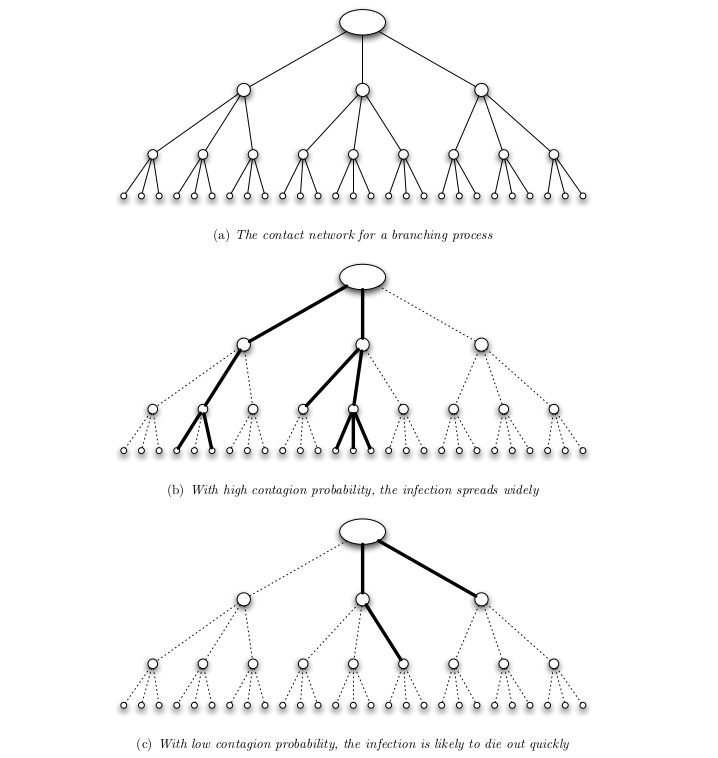
\includegraphics[width=.90\textwidth]{Figures/Selection_004.png}
	%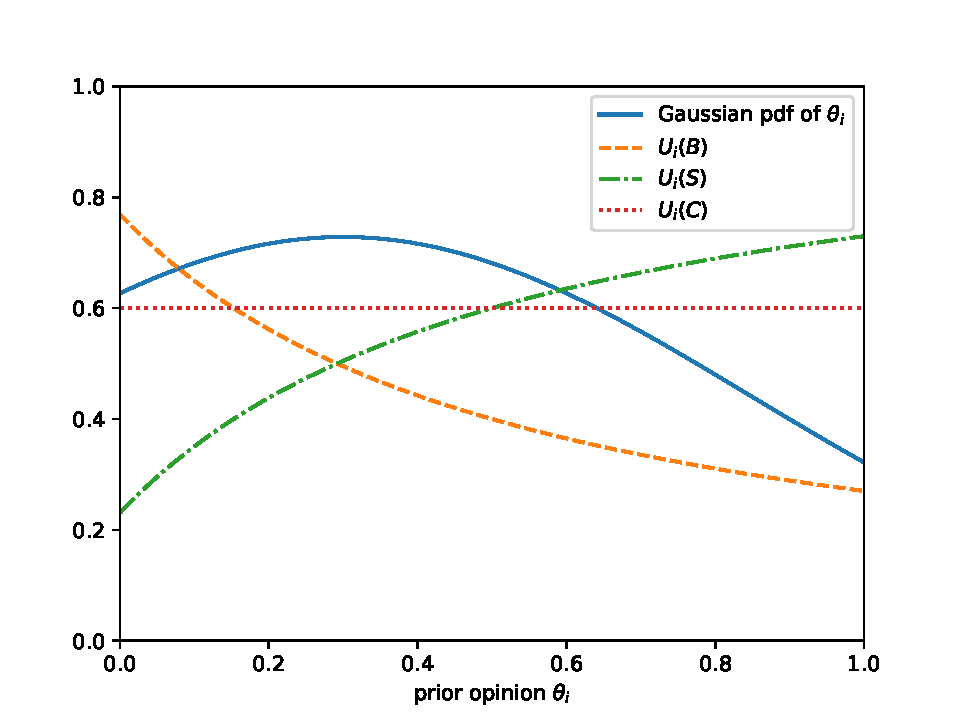
\includegraphics[width=.75\textwidth, height=.3\textheight]{Figures/line_plot.pdf}
	
	\caption{Branching process example with $k=3$. Reference in ~\cite{Kleinberg}.}
	
	\label{fig:branchProc}
\end{figure}

The above rules define a simple epidemic model where the probability of infections represents the rate and $k$ is the an average amount of a person's contacts. The question on those models is if the disease will survive (i.e., turn into a pandemic) or eventually stop spreading and die. The basic reproductive number determines whether a virus will continue spreading or if it fails. We have the next proposition from ~\cite{Kleinberg}:

\begin{prop}
	Let $R_0 = p k $ be the basic reproductive number where $k$ is the average people an individuals meets and $p$ is the probability that the virus spreads. If $R_0 \geq 1$, then with probability greater than zero the virus persists. If the basic reproductive number is less than $1$ then with probability $1$ the virus with stop spreading after some waves.
\end{prop}

The proof is provided more analytically in the related reference and it is based on geometric sequences, which will concern the more complex branching process later on the main body of this thesis. The reproductive number in our study can be translated as a prediction where we can tell if the process will trigger a cascade, given the contagion probability and the average people that a person \textit{meets}.

In our thesis we use a more complex version of that model. First of all, we do not have a fixed probability for infection. Every time nodes are added in the propagation tree, this probability is affected. Another modification we make on that model is the time that the process takes place. Instead of waves, we assume that each node contacts his neighbors at some time $t$, more later at the appropriate chapter. Although branching process seems significantly simpler than epidemics, it captures more with the correct modifications and that is the fact that it micro manage the contagion inside a network. In a nutshell, epidemics translate only the ratio at where entities move from a state to another and it does not account a change of probabilities.

\section{Bayesian Inference}
\label{sec:BayesianInf}

Bayesian inference is a statistical inference that update beliefs about uncertain parameters as more information becomes available. The Bayesian inference is one of the most successful methods used in decision theory, builds over Bayes’ theorem:
$$\mathbb{P}(H|E) = \frac{\mathbb{P}(E|H)\mathbb{P}(H)}{\mathbb{P}(E)}$$
which expresses the conditional probability of the hypothesis $H$ conditional to the event $E$ with the probability that the event, or evidence, $E$ occurs given the hypothesis $H$. In the previous expression, the posterior probability $\mathbb{P}(H|E)$ is inferred as an outcome of the prior probability $\mathbb{P}(H)$ on the hypothesis, the model evidence $\mathbb{P}(E)$ and the likelihood $\mathbb{P}(E|H)$ of the evidence $E$ occurring, given the validity of the hypothesis $H$. Bayes’ theorem has been widely used as an inductive learning model to transform prior and sample information into posterior information and is widely used in decision theory. In order to visualize the concept of Bayes theorem, we provide a simple example. Suppose people are tested for some disease. If the test is $99\%$ accurate, then this means that  $\mathbb{P}(Positive-test|Positive)  =  0.99$. However, the  most relevant information is $\mathbb{P}(Positive|Positive-test)$, namely the probability of having the disease if the test is positive, using Bayes theorem. If the proportion $\mathbb{P}(Positive)$ of infected people in the total population is $0.001$, then if we have the value of normalizing factor, i.e. $\mathbb{P}(Positive-test)=0.01$, and we conclude that $\mathbb{P}(Positive|Positive-test) = 0.099$, which provides different information and more relevant, using evidence rather than a simply using the accuracy of the test. It is obvious that both prior observations and the observable data, contain information, and so neither should be neglected. Bayes theorem has a general form as well, that works with multiple variables. The formula for discrete multiple variables, which we use in our thesis, is:

$$\mathbb{P}(H_k|E) = \frac{\mathbb{P}(E|H_k)\mathbb{P}(H_k)}{\sum_{i \in I} \mathbb{P}(E|H_i) \mathbb{P}(H_i)}$$
where ${H}_{i \in I}$ is partition of the sample space and $H_k$ is an observation inside that partition.

The process of drawing conclusions from available information is called inference.  However, in  many  cases the available information is often insufficient to  reach  certainty through reasoning.  In these cases, one may use different approaches for doing inductive inference. The strength of Bayesian inference, which is the method of using Bayes theorem to deduce a claim, is that it requires minimum but relevant information in order to work. This ability makes Bayesian inference an appropriate method to express how opinions are formed inside a social structure. Other notable applications are in medicine, machine learning, data analysis and many more. %Preliminaries 		 ch:2


\chapter{Agents Propagation Model}
\label{ch:Agents Propagation Model}

In this chapter we describe the information propagation process among a group of rational agents taking place in discrete time. We first provide a probabilistic representation of the information shared by this group of individuals under our assumptions followed by the propagation rules of our model. Finally, we conclude this chapter with an analysis of agents news-sharing process dynamics and the structural properties that arise from those. Although this thesis is provides all the basic background, we suggest the reader to study \cite{papanastasiou} which is the basis of our model.


\section{A Probabilistic Representation of News}
\label{sec:FKNews param}
We assume that each event in the world is characterized by a binary state $\Theta \in \{Y,N\}$ \footnote{This model supports events with more than two states but for the sake of simplicity we stay in a binary model.} which is unobservant by a group of individuals (we call them agents) and they are of interest to find the exact value of $\Theta$. Agents may create informative content in forms of news articles (we call them stories) that contain information over the ground truth. These stories are described by $m \in \{y,n\}$ and state the creators realization of the ground truth $\Theta$. Each story can be characterized by another unobservant variable $V \in \{F,T\}$ which declares the validity of its content. If the stance of a story aligns with the actual event, we have $V=T$ with respect to $\Theta$ (truthful story). In the other hand we have $V=F$ with respect to $\Theta$ (fake story) whenever we are dealing with stories that are uninformative or misleading in respect to $\Theta$. \footnote{We should mention that our model does not capture the intention of creating fake stories, i.e. deliberately creating fake information or bad journalism.} 

\begin{table}[t]\
\centering
\captionsetup{justification=centering}
\caption{The probability distribution of truthful stories ($V=T$ left) and fake stories($V=F$ right) with respect to the ground truth.}
\label{tab:Message Type}
\begin{tabular}{ l  l }
\begin{tabular}{| c || c | c |}
\hline
$P(m \mid ( \Theta , V) )$ & $\Theta = Y$ & $\Theta = N$ \\
\hline
\hline
$m=y$                    & $a$          & $1-a$        \\
\hline
$m=n$                    & $1-a$        & $a$         \\
\hline
\end{tabular}
&
\begin{tabular}{| c || c | c |}
\hline
$P(m \mid ( \Theta , V) )$ & $\Theta = Y$ & $\Theta = N$ \\
\hline
\hline
$m=y$                    & $\beta$          & $\beta$        \\
\hline
$m=n$                    & $1-\beta$        & $1-\beta$         \\
\hline
\end{tabular}
\end{tabular}
\end{table}

In table ~\ref{tab:Message Type} we have the probability distributions for both possible types of messages when we are characterizing them with their validity $V$. The signal-generating process for truthful stories is described by the system of equations:

\begin{align}
	\begin{split}
		\mathbb{P} ( y \mid (Y,T)) = \mathbb{P} ( n \mid(N,T)) &=a \\
		\mathbb{P} ( y \mid (N,T)) = \mathbb{P} ( n \mid(Y,T)) &=1-a
	\end{split}
\end{align}


where $a$ can be translated as the persuasiveness of source without any other prior knowledge (i.e. the sharing history) or the probability of a story that shares the same stance as the ground truth thus having truthful validity. We assume that the persuasiveness is $a \in (0.5,1)$ and it is known parameter in our ecosystem. On contrary, when we are dealing with fake stories the signal-generating process is:
\begin{align}
	\begin{split}
		\mathbb{P} ( y \mid (Y,F)) &= \mathbb{P} ( y \mid(N,F)) =\beta \\
		\mathbb{P} ( n \mid (Y,F)) &= \mathbb{P} ( n \mid(N,F)) =1-\beta
	\end{split}
\end{align}
From the above equations we notice that the probabilities of stories $m$ in both cases remain the same over different values of $\Theta$. This reflects the fact that the content of a story is totally uninformative and is randomly aligned with one of the possible states for ground truth, i.e if $\beta > 0.5$ the author of a the story pushes his own agenda with a false narrative described by a story of type $m=y$. Another observable variable, that we assume it is common knowledge, is the percentage of fake stories that circulate in our social infrastructure. Platform can monitor the validity of previous stories and calculate the frequency, or an approximation, of fake stories denoted as $v$. We can also express this quantity as the probability of a newly created story being fake without any prior evidence, $v= \mathbb{P} ( V=F )$. Those parameters conclude all possible outcomes of a message type, in terms of validity and stance, that describes a binary state of an event. In the next section we provide an example in order to illustrate how those parameters work in a real scenario.

\subsection{Example}
\label{subsec:exmpl}

We now provide an illustrative example in order to understand the role of those parameters named in the previous section. There are several real world incidents we can reference from fact checking sites, but we use a fabricated example for the sake of simplicity.~\footnote{Some examples fact checking sites are snopes \url{https://www.snopes.com/} and politifact \url{https://www.politifact.com/}.}

Suppose we have the next claim about COVID-19:

\textit{"University of Ioannina study finds that mortality rate of COVID-19 is lower in countries with warmer climate."}

In our example, we have the ground truth, described by $\Theta \in \{Y,N\}$ where $Y$ aligns with the content of the sentence, in other words $Y$ is interpreted as \textit{"Yes, mortality rate is lower in warmer climates"}, while $N$ presents no link between climate and the mortality rate of COVID-19. The content of the article support $\Theta = Y$ so we have that $m=y$. Also we expect that a claim made by university of Ioannina would be highly persuasive since it would be researched with valid methods so $a$ is expected to be over $85\%$, taken at face value. This means that we are likely to adopt the validity of that claim no matter the content of the research, only by attributing the persuasiveness of the source as an authoritative entity in the research domain. Another case is when we expect from the source of a story to be in interest to push a story that aligns with a narrative. For example, if we knew that university of Ioannina had benefit from supporting $Y$, then it might be the case that it produces a fake story, whose stance $m=y$ holds with probability $\beta$, independently of the actual value of the ground-truth variable $\Theta$. Another scenario is when we expect that the source is not biased but we distrust their journalistic effort or the claim is more likely to be false. Remember that $\beta$ expresses the bias of a source to produce a fake story that supports either $Y$ or $N$, while $\beta = 0.5 $ means that the fake story is produced randomly to align with one side.

Now let's assume that all stories circulating our social structure is probably truthful. This means that $v$ is approaching $0\%$ and in order to simplify things, let $v=0$. An agent with prior belief $\theta = \mathbb{P} (\Theta = Y)$ will update his posterior belief as:
$$\theta_{posterior} =  \mathbb{P} (\Theta = Y \mid m=y ) = \frac{a \theta}{a \theta +(1-a)(1-\theta)}$$
which is greater that his prior belief $\theta$ since $a \in (0.5,1)$. In other words, the fact that all stories are truthful strengthens agent posterior belief that $\Theta = Y$ or equivalent that the story is truthful, $V=T$ and $m=y$. On the contrary, if all the stories shared within the social network are almost certainly fake, $v=1$, we have that:
$$\theta_{posterior} = \frac{\beta \theta}{\beta \theta +(1-\theta)\beta}=\theta_{prior}$$
We see that posterior belief remains the same as our prior opinion since any new information over previous actions would not affect agents  posterior belief. 

\section{Sharing Process and Agents Behavior}
\label{sec:SharingProc}

We assume that a group of infinite rational agents act in a discrete time $t \in \{1,2,...\}$ (we refer time as round $t$) based on various parameters. Each agent is characterized by its own prior belief over ground truth which we assume that is an \textit{iid} draw from a Gaussian distribution. We denote agent $i$'s prior belief as $\theta_{i0} := \mathbb{P} ( \Theta = Y ) $. \footnote{Without loss of generality, we assume that prior opinions describe each agent's belief over one opinion, namely $\Theta = Y$. Proofs for theorems and corollaries in this work are similar for $\Theta = N$ and we mention if otherwise.} The process begins with an emerging story from the first node \footnote{We can assume that the first node is $i=0$ since we can rearrange those \textit{id's}, which is planted from an external source. We notice that $t$ and $i$ are similar in paths but this statement does not hold for other structures such as trees.}. Each agent can choose between the next strategies:

\begin{itemize}
	\item React to the story by sharing it to its out-neighbors (follower list), without inspecting its content. We refer to this action as \textbf{send}.
	\item Refuse to share the story, namely \textbf{block}, without checking the content.
	\item To \textbf{check} the story and choose one of the next actions:
	\begin{itemize}
		\item Share the story is she$\backslash$he finds that the article is truthful.
		\item Not share if she$\backslash$he finds that the story is fake.
	\end{itemize}
\end{itemize}

The strategy of each agent at round $t$ is denoted as $A_{it} = \{S,B,C\}$ for each of the above actions respectively. From the above strategies we can see that each one of them splits into 2 steps, namely the inspection choice and the sharing choice. We assume that if an agent picks $A_{it} = C$, the inspection yields a perfect result and the next action dependents on it, i.e. we have socially responsible agents that do not share fake stories. Thus we do not include the option to inspect and share a story if it is evaluated as fake. In advance, we mention that if an agent chooses to share the story either by \textbf{send} or \textbf{check}, we assume that he shares the message by broadcasting to a group of agents as we see in figure ~\ref{fig:broadcast}. Next, we define the probabilities of the above actions in strategy set $A_{it}$, as:

\begin{definition}
	\label{def:ActionProbabilities}
	The probabilities of each action $A_{it}$ that agent $i$ selects at round $t$ are:
	\begin{itemize}
		\item $S_{it} = \mathbb{P}_{i} \{A_{it} = S \mid m=y , H_i\}$
		\item $B_{it} = \mathbb{P}_{i} \{A_{it} = B \mid m=y , H_i\}$
		\item $C_{it} = \mathbb{P}_{i} \{C_{it}= C \mid m=y , H_i\}$ and $C_{it} = 1-S_{it}-B_{it} $
	\end{itemize}for actions $\{S,B,C\}$ respectively.
\end{definition}
In the analysis of this chapter about agents' sharing process dynamics, we provide closed form equations of the above probabilities.

\begin{figure}
		\definecolor {processblue}{cmyk}{0.96,0,0,0}
		\definecolor {processred}{cmyk}{0.96,0,0,0}
		\tikzstyle{c} = [thick,draw, circle, minimum size=2,top color =white ,minimum size=2, bottom color = processblue!20,processblue]
	\centering
	\begin{tikzpicture}[main/.style={c},
		level distance=15mm,
		level 1/.style={sibling distance=20mm},
		level 2/.style={sibling distance=30mm},
		level 3/.style={sibling distance=15mm},
		end/.style = {draw, circle, minimum size=2,fill,top color=white,bottom color=red!20,red},
		discovered/.style = {draw, circle, minimum size=2,fill,color = red}]
		\node (a)[main,label=left:{$\theta_1$}]{}[edge from parent]
		child {
			node (b) [end,label=left:{$\theta_2$}]{}
		}
		child {
			node (c)[end,label=left:{$\theta_3$}]{} 
		}
		child {
			node (d)[end,label=left:{$\theta_4$}]{} 
		}	
		child {
		node (e) [end,label=left:{$\theta_5$}]{} 
		};
		\draw (a) -- (b) node [midway, fill=white] {S};
		\draw (a) -- (c) node [midway, fill=white] {S};
		\draw (a) -- (d) node [midway, fill=white] {S};
		\draw (a) -- (e) node [midway, fill=white] {S};
	\end{tikzpicture}
	\caption{Agent $\theta_1$ shares by sending without checking $(A_{1t}=S)$ the story via broadcast to a group of agents (red).}
	\label{fig:broadcast}
\end{figure}

At each round, we assume that an agent acts and picks one of the actions mentioned in the previous paragraph. This sequential process forms a sub-network $G' \subseteq G$ of the original network $G=(V,E)$. We refer this sub-graph as \textit{sharing sub-network} or \textit{sharing tree}, when we are dealing with tree structures, and this sub-graph is known to the platform. For agent $i$ we assume that the \textit{sharing history} he perceives, namely $H_i$, is the unique path from the originator of the story (source) up to agent $i$. As we see in figure ~\ref{fig:histories}, we have the sharing network in which the red edges indicate the sharing history for agent $k$, with prior belief $\theta_k$, in a path and a tree. The sharing network and history for agent $i$ are the same for a path in contrast with a tree, where we assume that agent $i$ knows that the story is shared only by his predecessors. In our analysis we assume that if agent $i$ receives a story from a agent $j$, he cannot receive the same story from another node $l$. As we see in figure ~\ref{fig:histories}, $\theta_5$ receives the story from $\theta_2$ thus $\theta_3$ will not broadcast the story to $\theta_5 $ again.\footnote{We make a discussion for DAG's in general in a final chapter of this thesis.}

\begin{figure}
	\definecolor {processblue}{cmyk}{0.96,0,0,0}
	\definecolor {processred}{cmyk}{0.96,0,0,0}
	\centering
\begin{subfigure}{1\linewidth}
	\centering	
	\begin{tikzpicture}[node distance={26mm}, thick, main/.style = {draw, circle, minimum size=2,top color =white , bottom color = processblue!20 ,draw,processblue},end/.style ={draw, circle, minimum size=2,fill,top color=white,bottom color=red!20,red}]
			\node[main,label=below: {$\theta_1$}] (1) {}; 
			\node[main,label=below:{$\theta_2$}] (2) [right of=1] {};
			\node[main,label=below:{$\theta_3$}] (3) [right of=2] {};
			\node[main,label=below:{$\theta_4$}] (4) [right of=3] {};
			\node[main,label=below:{$\theta_{k-1}$}] (5) [right of=4] {};
			\node[end,label=below:{$\theta_k$}] (6) [right of=5] {};
			
			\draw[->,color=red] (1) -- (2);
			\draw[->,color=red] (2) -- (3);
			\draw[->,color=red] (3) -- (4);
			\path (4) -- node[auto=false]{\ldots} (5);
			\draw[->,color=red] (5) -- (6);		
		\end{tikzpicture}
		\subcaption{Sharing path}
\end{subfigure}
\begin{subfigure}{1\linewidth}
	\centering
	\tikzstyle{c} = [thick,draw, circle, minimum size=2,top color =white ,minimum size=2, bottom color = processblue!20,processblue]
		\begin{tikzpicture}[main/.style={c},
			level distance=15mm,
			level 1/.style={sibling distance=60mm},
			level 2/.style={sibling distance=30mm},
			level 3/.style={sibling distance=15mm},
			end/.style = {draw, circle, minimum size=2,fill,top color=white,bottom color=red!20,red},
			discovered/.style = {draw, circle, minimum size=2,fill,color = red}]
			\node (a)[main,label=left:{$\theta_1$}]{}[edge from parent]
			child {
				node (b) [main,label=left:{$\theta_2$}]{}
				child {node [main,label=left:{$\theta_4$}]{}
					child{ node  [main,label=left:{$\theta_8$}]{} }
					child{ node [main,label=left:{$\theta_9$}]{} }
				}
				child {node (c) [main,label=left:{$\theta_5$}]{}
					child{ node [main,label=left:{$\theta_{10}$}]{} }
					child{
						node (d) [end,label=left:{$\theta_{11}$}]{}
						child{ node [main,label=left:{$\theta_{14}$}]{} }
						child{ node [main,label=left:{$\theta_{15}$}]{} }
					}
				}
			}
			child {node (e) [main,label=left:{$\theta_3$}]{} 
				child {node [main,label=left:{$\theta_6$}]{}
					child{ node [main,label=left:{$\theta_{12}$}]{} }
					child{ node [main,label=left:{$\theta_{13}$}]{} }
				}
				child {node [main,label=left:{$\theta_7$}]{}
				}		
			};
			\draw [->,color=red] (a) -- (b);
			\draw [->,color=red] (b) -- (c);
			\draw [->,color=red] (c) -- (d);
			\draw [->,dashed] (e) -- (c);
		\end{tikzpicture}
		\subcaption{Sharing Tree}
\end{subfigure}
		\caption{Sharing process of a story in different structures (a) Path and (b) Binary tree.}
		\label{fig:histories}
\end{figure}

Throughout the process, agents form and update their beliefs about the validity of the story that is being shared in the network, and their validity. There are two basic probabilities that express the agents opinions. First, we have the agents' own posterior belief over the value of ground-truth as well the agents' posterior belief that an article is fake, respectively: 
\begin{equation}\label{eq:beliefs}
	\begin{split}
		b_{it} = P_i \{ \Theta = Y | m = y , H_i \} \\
		q_{it} = P_i \{ V=F | m = y , H_i \}
	\end{split}
\end{equation}
where he receives a message $m=y$ with a history path $H_i$, $\forall t \geq 0$. At each given round $t$ agent updates his own posterior beliefs based on a group of parameters that is common knowledge. The parameters that each agents knows at the round $t$, when he receives the story are:

\begin{itemize}
	\item The sharing history $H_i$ up to him from the source.
	\item His own prior belief $\theta_i$ for the ground-truth.
	\item The ratio of fake news and truthful news that circulate in the platform annotated as $v$.
	\item The credibility $a$ of a true story delivering a correct message about the ground-truth value. 
	\item The probability $\beta$ that a fake story promotes the stance $m=y$ for the  ground-truth variable, irrespectively of its actual value.   
\end{itemize}
With the list of above parameters we calculate the closed form equations for ~\ref{eq:beliefs} that are the posterior beliefs of an agent $i$.
\begin{prop}
	For each $i$ agent at each round $t \geq 0$ it holds that:
	$$b_{it} = \mathbb{P}_i \{ \Theta = Y | m = y , H_i \} =  \frac{\theta_i[\beta v w_{it}+a(1-v)]}{\beta v w_{it} + [a \theta_i + (1-a)(1-\theta_i)](1-v)}$$
	$$q_{it} = \mathbb{P}_i \{ V=F | m = y , H_i \} = \frac{\beta v w_{it}}{\beta v w_{it} + [a \theta_i + (1-a)(1-\theta_i)](1-v)}$$
where $w_{it} = \displaystyle\prod_{k=0}^{t-1} \frac{S_{ik}}{S_{ik}+C_{ik}}$ and $w_{i0} = 1$
\label{prop:beliefs}
\end{prop}

\begin{proof}
We construct the equation for $q_{it}$ since it is the main quantity that we will consider mostly in our work and the proof for $b_{it}$ is equivalent. 
The beliefs of this model are defined over the set $G =\{(\Theta , V )\}_{\Theta \in \{Y,N\},V \in \{T,F\}}$ and according to our model for fake news and the independence of $V$ and $\Theta$, we have the prior opinions of an agent as:
	\begin{itemize}
		\item $\mathbb{P}_{i0} \{(Y,T)\} = \theta_i (1-v) $
		\item $\mathbb{P}_{i0} \{(Y,F)\} = \theta_i v $
		\item $\mathbb{P}_{i0} \{(N,T)\} = (1-\theta_i) (1-v) $
		\item $\mathbb{P}_{i0} \{(N,F)\} = (1-\theta_i) v $
	\end{itemize}
Suppose an agent $i$ receives a story in round $t$, he uses all the information available to him in order to form his posterior belief that a story is fake. The only quantity that changes as time passes is $H_i$. For an opinion $g \in G$ we have the agents' posterior belief:
\begin{equation}
	\begin{split}
		\mathbb{P}_{it} \{g \mid m=y , H_i\} = \frac{\mathbb{P}_{} \{m=y , H_i \mid g\}\mathbb{P}_{} (g)}{\displaystyle\sum_{g' \in G}^{}\mathbb{P}_{} \{m=y , H_i \mid g'\}\mathbb{P}_{} (g')} = 
		\\ =\frac{\mathbb{P}_{} \{ H_i \mid m=y , g\} \mathbb{P}_{} \{ m=y \mid  g\} \mathbb{P}_{} (g)}{\displaystyle\sum_{g' \in G}^{}\mathbb{P}_{} \{ H_i \mid m=y , g'\} \mathbb{P}_{} \{ m=y \mid  g'\} \mathbb{P}_{} (g')}
	\end{split}
\end{equation}
which is the generalized Bayesian inference of an opinion $g$ among a set of opinions $G$. Now we calculate each probability in that expression in order to form $q_{it}$. From section ~\ref{sec:FKNews param} we have the probabilities below:
$$\mathbb{P}_{} \{ m=y \mid (Y,T)\} = a, \mathbb{P}_{} \{ m=y \mid (N,T)\} = 1-a,$$
$$ \mathbb{P}_{} \{ m=y \mid (N,F)\} = \mathbb{P}_{} \{ m=y \mid (Y,F)\} = \beta$$
Now we calculate the quantity $\mathbb{P}_{} \{ H_i \mid m=y , g\}$ which is the probability of a history given a $m=y$ story and an opinion. We are given that the story is $y$, thus agent $i$ considers his strategy only on $V$. This means that a fake story is shared only by action $S$ and a truthful story either by $S$ or $C$:
$$\mathbb{P}_{} \{ H_i \mid m=y , (Y,F)\} = \mathbb{P}_{} \{ H_i \mid m=y , (N,F)\} = $$ $$ \displaystyle\prod_{k=0}^{t-1}\mathbb{P}_{} \{ A_{it}=S \mid m=y , H_i\} =S_{it}$$ 
and
$$\mathbb{P}_{} \{ H_i \mid m=y , (Y,T)\} = \mathbb{P}_{} \{ H_i \mid m=y , (N,T)\} = $$ $$ =\displaystyle\prod_{k=0}^{t-1} [\mathbb{P}_{} \{ A_{it}=S \mid m=y , H_i\} + \mathbb{P}_{} \{ A_{it}=C \mid m=y , H_i\} ]= S_{it} +C_{it}$$
Combining all the above equations, we can compute $q_{it}$:

\begin{align*}
	\begin{split}
		q_{it} & = \mathbb{P}_{it} \{g \mid m=y , H_i\} = \mathbb{P}_{it} \{(Y,F) \lor (N,F) \mid m=y , H_i\} = \\
		& = \frac{\beta v w_{it}}{\beta v w_{it} + [a \theta_{i0}+(1-a)(1-\theta_{i0})](1-v)}
	\end{split}	
\end{align*}
Using the above calculations we can calculate $b_{it}$ in the same way as:

\begin{align*}
	\begin{split}
		b_{it} & = \mathbb{P}_{it} \{g \mid m=y , H_i\} = \mathbb{P}_{it} \{(Y,T) \lor (Y,F) \mid m=y , H_i\} = \\
		& = \frac{\theta_i[\beta v w_{it}+a(1-v)]}{\beta v w_{it} + [a \theta_i + (1-a)(1-\theta_i)](1-v)}
	\end{split}	
\end{align*}
where $w_{it} = \displaystyle\prod_{k=0}^{t-1} \frac{S_{ik}}{S_{ik}+C_{ik}}$, $w_{i0} = 1$ is the proportion probability that a story creates a sharing tree $G'$ that is made with $A_{it} = S$ up to round $t$ where $S_{ik}$ and $C_{ik}$ are given by definition ~\ref{def:ActionProbabilities}.
 
\end{proof}

Throughout the sharing process, each agent acts only once and he receives the appropriate reward for his action. We define the utility of agent $i$, over his action $A$, the function $U_i(A_{it})$. Agent $i$ receives reward either if he blocks a fake story or chooses to share a truthful story. On the other hand, he receives no reward if he blocks a truthful story or shares a fake story. Finally, an agent that chooses to inspect a story, does so by paying a price. Notice that the above function is evaluated only for the variables $V$ and $A_{it}$. Collectively, the induced evaluation function is the following:

\begin{equation}
U_i(A_{it}) = 
\begin{cases}
	1, & (A_{it} = S \land V=T) \lor (A_{ih} = B \land V=F) \\
	0, & (A_{it} = B \land V=T) \lor (A_{ih} = S \land V=F) \\
	1-K, & A_{it} = C \\
\end{cases} 
\end{equation}
where $K$ is the cost of inspection. We assume that inspection occurs with a cost $K < 0.5$ to avoid trivial cases where inspection is never optimal strategy. Agents are choosing actions that maximize their utility at $t$-round and in order to do so, they rely on their beliefs for values about the ground truth that we defined in proposition ~\ref{prop:beliefs}. Each agent chooses the strategy that maximizes his expected utility, given his belief that the story is fake, $q_{it}$. The expected utility can be calculated with the next proposition: 

\begin{prop}
	The expected utility of agents action is given by the function:
	$$\mathbb{E} [U_i(A_{ih})] = 
	\begin{cases}
		1-q_{ih}, & A_{ih} = S  \\
		q_{ih}, & A_{ih} = B  \\
		1-K, & A_{ih} = C \\
	\end{cases} $$
	\label{prop:ExpUtility}
\end{prop}

\begin{proof}
	And agent receives reward if he shares truthful stories or blocks fake according to his belief. Thus, agents $j$ expectation for action send, according to his belief $q_{jt}$  in round $t$, is $\mathbb{E} [U_j(S)] =  (1-q_{jt}) U_j (S \land T) + q_{jt} U_j (S \land F)=1-q_{jt}$. In similar manner we have that expected utility gained from blocking a story, based on agents $j$ belief that is fake, is $\mathbb{E} [U_j(S)] =  (1-q_{jt}) U_j (B \land T) + q_{jt} U_j (B \land F)=q_{jt}$. Finally, if a rational agent chooses to inspect a story based on his updated belief, the expected utility can be calculated as $\mathbb{E} [U_j(C)] =  (1-q_{jt}) U_j (S \land T) + q_{jt} U_j (B \land F)-K=1-q_{jt}+q_{jt}-K=1-K$ where the subtraction of $K$ presents the cost that agent $j$ pays in order to inspect a story and decide whether to send a truthful story or block it otherwise.
\end{proof}

In figure ~\ref{fig:utilities} we have an illustration of the utility curves over different values of $\theta_i$. Figure ~\ref{fig:utilities} is also a visual justification for the assumption that we made for $K < 0.5$. We can clearly see that if we assigned a value greater than $0.5$, then $1-K<0.5$ which implies that $U_i(B) > U_i(C)$, $\forall \theta_i \in (0,\overline{\theta})$ where $U_i(B)$ and $U_i(S)$ intersect, and after that point it holds that $U_i(S) > U_i(C)$,  $\forall \theta_i \in (\mu,1)$.

\begin{figure}[t]
\centering
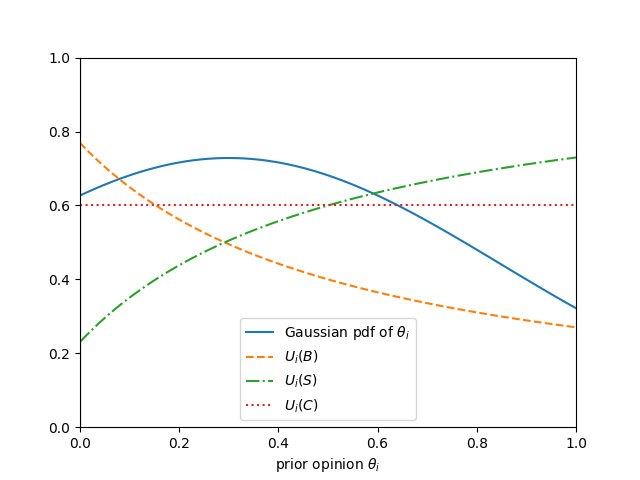
\includegraphics[width=.75\textwidth]{Figures/utilities.png}
%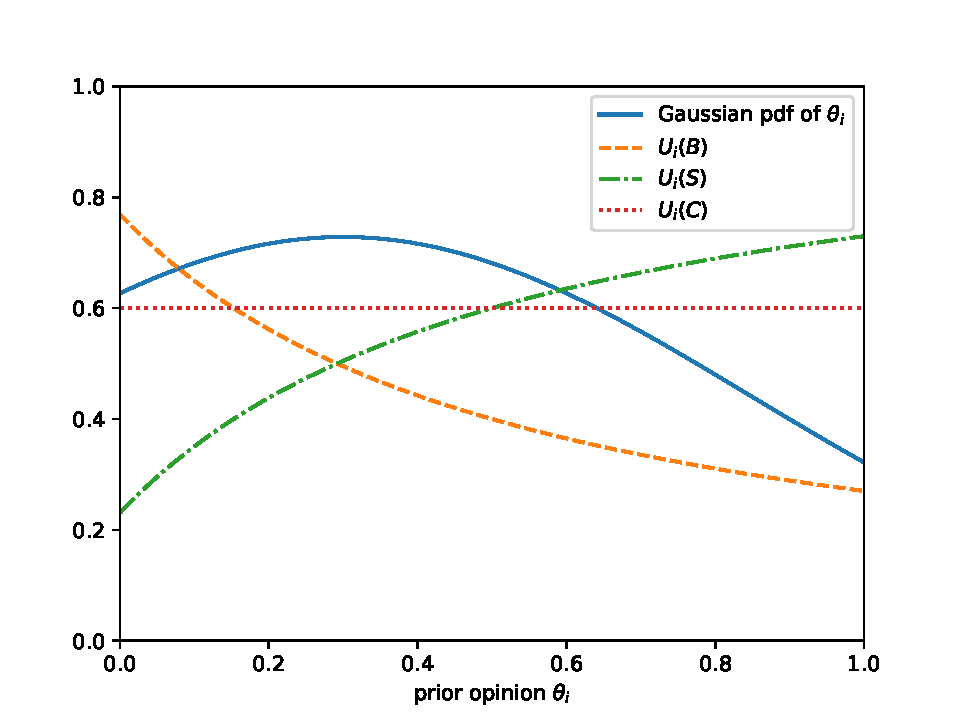
\includegraphics[width=.75\textwidth, height=.3\textheight]{Figures/line_plot.pdf}

\caption{The expected utility curves over different prior beliefs that follow a Gaussian distribution at first round. Parameters: $v=K=0.4$, $a=90\%$ and $\theta_i \sim \mathcal{N} (\mu=0.3,\sigma^2=0.09)$.}

\label{fig:utilities}
\end{figure}

\section{Propagation Dynamics}
\label{ch:Dynamics}

In this section we will focus on the dynamics of agents propagation and the properties of our setup, in order to help us tackle the main problem which is the optimal time that we can intervene to stop the propagation of a fake story. In order to introduce the properties, we describe each individual step of the process in a sharing tree. The proofs for theorems, propositions and lemmas that are mentioned in related work are provided in ~\ref{app:AppendixA}.

At each round $t$ an agent $i$ is up to decide if he will inspect a story $m=y$ and then if he will share it via a broadcast on a group of agents, i.e. his followers.\footnote{The choice of agents that are going to react and how it affects the sharing tree and the inspection time is further studied later on this thesis.} According to his belief, he evaluates each strategy and picks the one with that maximizes his expected utility. If he decides to share the story, he broadcasts the story to the set of all its out-neighbors (i.e., his$\backslash$her followers) in the underlying social-network graph. In round $t+1$, we pick another agent to act in a sense that round $t$ is a counter that determines how many agents have reacted. On the other hand, if an agent $j$ decides to not share the story, no matter if he inspects or not, the sharing history $H_j$ is discontinued at his path. Notice that in case of paths, time and agents are equivalent in the sense that we can refer to each agent as $t$ agent that is up to act. Additionally, if an agent decides not to share the story, the whole process is discontinued while in an $m$-ary tree it stops only in the particular sub-tree whose root node decides not to share. 

\begin{figure}
	\definecolor {processblue}{cmyk}{0.96,0,0,0}
	\definecolor {processred}{cmyk}{0.96,0,0,0}
	\tikzstyle{c} = [thick,draw, circle, minimum size=2,top color =white ,minimum size=2, bottom color = processblue!20,processblue]
	\begin{minipage}{.3\textwidth}
		\subcaption{}
		\begin{tikzpicture}[main/.style={c},
			level distance=15mm,
			level 1/.style={sibling distance=30mm},
			level 2/.style={sibling distance=20mm},
			level 3/.style={sibling distance=10mm},
			end/.style = {draw, circle, minimum size=2,fill,top color=white,bottom color=red!20,red},
			discovered/.style = {draw, circle, minimum size=2,fill,color = red}]
			\node (1)[main,label=left:{$\theta_1$}]{}[edge from parent]
			child {
				node (2) [main,label=left:{$\theta_2$}]{}
			}
			child {
				node (3)[main,label=left:{$\theta_3$}]{} 
			};
			
			\draw (1) -- (2) node [midway, fill=red] {S};
			\draw (1) -- (3) node [midway, fill=red] {S};
		\end{tikzpicture}
		
	\end{minipage}
	\begin{minipage}{.3\textwidth}
		\subcaption{}
		\begin{tikzpicture}[main/.style={c},
			level distance=15mm,
			level 1/.style={sibling distance=30mm},
			level 2/.style={sibling distance=20mm},
			level 3/.style={sibling distance=10mm},
			end/.style = {draw, circle, minimum size=2,fill,top color=white,bottom color=red!20,red},
			discovered/.style = {draw, circle, minimum size=2,fill,color = red}]
			\node (1)[main,label=left:{$\theta_1$}]{}[edge from parent]
			child {
				node (2) [main,label=left:{$\theta_2$}]{}
				child {
					node (4) [main,label=left:{$\theta_4$}]{}
				}
				child {
					node (5)[main,label=left:{$\theta_5$}]{}
				}
			}
			child {
				node (3)[main,label=left:{$\theta_3$}]{} 
			};
			\draw (1) -- (2) node [midway, fill=white] {S};
			\draw (1) -- (3) node [midway, fill=white] {S};
			\draw (2) -- (4) node [midway, fill=red] {S};
			\draw (2) -- (5) node [midway, fill=red] {S};
		\end{tikzpicture}
		
	\end{minipage}
	\begin{minipage}{.3\textwidth}
		\subcaption{}
		\begin{tikzpicture}[main/.style={c},
			level distance=15mm,
			level 1/.style={sibling distance=30mm},
			level 2/.style={sibling distance=20mm},
			level 3/.style={sibling distance=14mm},
			end/.style = {draw, circle, minimum size=2,fill,top color=white,bottom color=red!20,red},
			discovered/.style = {draw, circle, minimum size=2,fill,color = red}]
			\node (1)[main,label=left:{$\theta_1$}]{}[edge from parent]
			child {
				node (2) [main,label=left:{$\theta_2$}]{}
				child {
					node (4) [main,label=left:{$\theta_4$}]{}
				}
				child {
					node (5)[main,label=left:{$\theta_5$}]{}
					child {node (6)[main,label=left:{$\theta_6$}]{}}
					child {node (7)[main,label=left:{$\theta_7$}]{}}
				}
			}
			child {
				node (3)[main,label=left:{$\theta_3$}]{} 
			};
			
			\draw (1) -- (2) node [midway, fill=white] {S};
			\draw (1) -- (3) node [midway, fill=white] {S};
			\draw (2) -- (4) node [midway, fill=white] {S};
			\draw (2) -- (5) node [midway, fill=white] {S};
			\draw (5) -- (6) node [midway, fill=red] {S};
			\draw (5) -- (7) node [midway, fill=red] {S};
		\end{tikzpicture}
		
	\end{minipage}
	\begin{minipage}{.5\textwidth}
		\subcaption{}
		\begin{tikzpicture}[main/.style={c},
			level distance=15mm,
			level 1/.style={sibling distance=30mm},
			level 2/.style={sibling distance=20mm},
			level 3/.style={sibling distance=10mm},
			end/.style = {draw, circle, minimum size=2,fill,top color=white,bottom color=red!20,red},
			discovered/.style = {draw, circle, minimum size=2,fill,color = red}]
			\node (1)[main,label=left:{$\theta_1$}]{}[edge from parent]
			child {
				node (2) [main,label=left:{$\theta_2$}]{}
				child {
					node (4)[main,label=left:{$\theta_4$}]{}
				}
				child {
					node (5)[main,label=left:{$\theta_5$}]{}
					child {node (6)[main,label=left:{$\theta_6$}]{}}
					child {node (7)[main,label=left:{$\theta_7$}]{}}
				}
			}
			child {
				node (3)[main,label=left:{$\theta_3$}]{}
				child {node (8)[main,label=above left:{$\theta_8$}]{}}
				child {node (9)[main,label=left:{$\theta_9$}]{}}
			};
			
			\draw (1) -- (2) node [midway, fill=white] {S};
			\draw (1) -- (3) node [midway, fill=white] {S};
			\draw (2) -- (4) node [midway, fill=white] {S};
			\draw (2) -- (5) node [midway, fill=white] {S};
			\draw (5) -- (6) node [midway, fill=white] {S};
			\draw (5) -- (7) node [midway, fill=white] {S};
			\draw (3) -- (8) node [midway, fill=green] {C};
			\draw (3) -- (9) node [midway, fill=green] {C};
		\end{tikzpicture}
		
	\end{minipage}
	\begin{minipage}{.5\textwidth}
		\centering
		\subcaption{}
		\begin{tikzpicture}[main/.style={c},
			level distance=15mm,
			level 1/.style={sibling distance=30mm},
			level 2/.style={sibling distance=20mm},
			level 3/.style={sibling distance=14mm},
			end/.style = {draw, circle, minimum size=2,fill,top color=white,bottom color=red!20,red},
			discovered/.style = {draw, circle, minimum size=2,fill,color = red}]
			\node (1)[main,label=left:{$\theta_1$}]{}[edge from parent]
			child {
				node (2) [main,label=left:{$\theta_2$}]{}
				child {
					node (4)[main,label=left:{$\theta_4$}]{}
				}
				child {
					node (5)[main,label=left:{$\theta_5$}]{}
					child {node (6)[main,label=left:{$\theta_6$}]{}}
					child {node (7)[main,label=left:{$\theta_7$}]{}}
				}
			}
			child {
				node (3)[main,label=left:{$\theta_3$}]{}
				child {node (8)[main,label=above left:{$\theta_8$}]{}}
				child {node (9)[main,label=left:{$\theta_9$}]{}
					child {node (10)[main,label=left:{$\theta_{10}$}]{}}
					child {node (11)[main,label=left:{$\theta_{11}$}]{}}
				}
			};
			
			\draw (1) -- (2) node [midway, fill=white] {S};
			\draw (1) -- (3) node [midway, fill=white] {S};
			\draw (2) -- (4) node [midway, fill=white] {S};
			\draw (2) -- (5) node [midway, fill=white] {S};
			\draw (5) -- (6) node [midway, fill=white] {S};
			\draw (5) -- (7) node [midway, fill=white] {S};
			\draw (3) -- (8) node [midway, fill=white] {C};
			\draw (3) -- (9) node [midway, fill=white] {C};
			\draw (9) -- (10) node [midway, fill=red] {S};
			\draw (9) -- (11) node [midway, fill=red] {S};
		\end{tikzpicture}
		
	\end{minipage}
	\caption{The resulting sharing tree after five reactions, from $(a)$ to $(e)$.}
	\label{fig:SharingProcc}
\end{figure}

Before we further continue our study, it is time to illustrate each individual step of a sharing process with an extended example. Using figure ~\ref{fig:SharingProcc}, we begin with agent $1$ with $\theta_1$ that chooses to share the story $m=y$ with his neighbors. In order to do that, evaluates his expected utility for each action and picks the appropriate that has the maximum value. In order to do so, he calculates his posterior belief. In the beginning of the process, there is no sharing history since he is the first that reacts to the story on his unique path from the source up to him (i.e. he is the root). From proposition ~\ref{prop:beliefs} we have that $q_{11}= \displaystyle\frac{\beta v w_{11}}{\beta v w_{11} + [a \theta_{1}+(1-a)(1-\theta_{1})](1-v)}$ where $w_{11}=S_0/(S_0+C_0)$ since there is no previous sharing history. Continuing with the next agent $ \theta_2$ in $(b)$ he also evaluates his own posterior belief with the expected utility and he finds that it maximizes when he chooses to share with out checking as well. The difference this time is that the sharing history of his ancestors is non trivial, thus he has to make an estimation about $w_{it}$. In order to do so, he must calculate $w_{22} = \displaystyle\prod_{k=0}^{1} \frac{S_{ik}}{S_{ik}+C_{ik}}$ which translates to the probability \textit{that a story reaches to agent $i$ without any inspection} and it is a proportion of $q_{it}$. We notice that this quantity demands the knowledge of probabilities that concern the sharing actions of previous agents in his sharing history. It is obvious that if agent $i$ knew the prior beliefs of their ancestors, then agent $i$ would have a best response strategy and the choice of action would be deterministic. Since we want to study a model that works under uncertainty, we introduce the next two assumptions:
\begin{assumption}
Aside for the parameters that we assumed in section ~\ref{sec:SharingProc} is shared throughout all agents and in order for agent to update his belief by calculating $w_{it} = \displaystyle\prod_{k=0}^{t-1} \frac{S_{ik}}{S_{ik}+C_{ik}}$, we have two options:
	\begin{itemize}
		\item Agents presume that all prior opinions follow a normal distribution, $\theta_i \sim \mathcal{N} (\theta^*,\sigma^2)$, and $\theta^*$ is common knowledge in our social network $\forall i$.
		\item Agents presume that all prior opinions follow a normal distribution and each agent creates his own normal distribution centralized around him such that $\theta_j \sim \mathcal{N}_i (\theta^*,\sigma^2)$ with $\theta^* = \theta_i$, $\forall j$.
	\end{itemize}
\label{assum:AgentsPerceptionOfThetas}
\end{assumption}
The first option translates to a setup that agents determine past reactions based on a average prior opinion, i.e. an average value based on a similar subject that platform historically recorded in the social network. This approach creates a normalized sharing behavior because agents are assumed to be completely homogeneous, in the sense that they all sample exactly the same distribution when considering the prior beliefs of other agents. On the other hand, when agent $i$ uses his prior opinion to determine the reaction history up to him, e centers the normal distribution for sampling the other agents' prior beliefs to its own (actual) prior belief. I.e., the agents are now assumed to be heterogeneous.

Continuing in figure ~\ref{fig:SharingProcc}, at $(d)$ and $(e)$ derived sub-trees in our sharing process, we see that agent $\theta_3$ is choosing to inspect the information and share it with his neighbors, $\theta_8$ and $\theta_9$. For our model, and since we assumed that the inspection yields perfect outcome, it is sufficient to find an agent that inspected the story and chose to share it. This observation is useful in the next chapter that is focused on platform's inspection problem and the solution of interrupting probable viral stories that are shared with suspicious reactions.

In order to separate the actual probabilities that an agent $i$ chooses a strategy between $\{B,C,S\}$ from his estimated value about those probabilities for his ancestors, we introduce the next annotations:

\begin{definition}
	We define as $B_{it}^j,C_{it}^j,S_{it}^j$ the probabilities that agent $i$ observes for agent $j$ and his actions $\{B,C,S\}$ respectively for round $t$. More specifically, we have the equations below:
		$$B_{it}^j=\mathbb{P}_{i} \{A_{jt}(\theta_i^*) = B \mid m=y , H_j\}$$
		$$C_{it}^j=\mathbb{P}_{i} \{A_{jt}(\theta_i^*) = C \mid m=y , H_j\}$$
		$$S_{it}^j=\mathbb{P}_{i} \{A_{jt}(\theta_i^*) = S \mid m=y , H_j\}$$
where $A_{jt}(\theta_i^*)$ is the action that agent $i$ believes that is optimal for agent $j$ according to the assumption ~\ref{assum:AgentsPerceptionOfThetas} where agent $i$ presumes that his predecessors acting with some prior $\theta^*$.
\label{def:PresumedActionProbs}
\end{definition}

Now we provide closed form equations for probabilities in definitions ~\ref{def:ActionProbabilities} and ~\ref{def:PresumedActionProbs}, derived from the above proposition.
\begin{prop}
	Let be agent $i$ that is up to react in round $t$. Then for the probabilities $B_{it},C_{it},S_{it}$ it holds that:
	$$B_{it} = \mathcal{F} \left( \displaystyle\frac{1}{2\alpha-1}\left[\frac{\beta v w_{it} K}{(1-v)(1-K)}-(1-\alpha)\right] \right)$$

	$$S_{it} = 1-\mathcal{F} \left( \displaystyle\frac{1}{2\alpha-1}\left[\frac{\beta v w_{it} (1-K)}{(1-v)K}-(1-\alpha)\right] \right)$$  
	
	$$C_{it} = 1-B_{it}-S_{it}$$
where $\mathcal{F}$ is the cumulative distribution function (cdf) from where $\theta_i$'s are drawn. 
\label{prop:CloseProbabilitiesActions}
\end{prop}

It is important to notice that in proposition ~\ref{prop:CloseProbabilitiesActions}, the formulation is independent of the cdf $\mathcal{F}$ that distribution has. In our model we assumed that tall the agents, and the platform, presume that the other agents' prior beliefs are drawn independently from a normal distribution $N(\mu,\sigma^2)$

$$\mathcal{F}(x) = \frac{1}{2} \left[1+erf\left(\frac{x-\mu}{\sigma \sqrt{2}}\right)\right]$$
where $erf(x)$ is the error function specified in the background.

Now that we have the appropriate tools and specified the all the assumptions about how an agent processes information and how he acts, we are ready to analyze each component of our setup and find useful properties that will help us tackle the platform's inspection problem. One important property that will help in the analysis of this model is the monotonicity of $q_{it}$. The following lemmas from ~\cite{papanastasiou} are useful tools throughout the analysis.

\begin{lemma}
	Suppose that an agent receives a story in round $t$. The agent's posterior belief that the story is fake, $q_{it}$, is strictly decreasing in her prior opinion over ground truth, $\theta_i$.
	\label{lemma:prior}
\end{lemma}
\begin{lemma}
	Suppose that an agent receives a story in round $t$ with a sharing history $H_i$ and a prior belief over $\Theta$, $\theta_i$. The agent's posterior belief that this story is fake is decreasing as $t$ increases.
	\label{lemma:monotontime} 
\end{lemma}
The probability $q_{it}$ can be seen as a sequence of $\theta_i$, $\{q_{it}\}_{\theta_i \sim \mathcal{N} (\mu, \sigma)}$ for fixed $t$'s, or as a sequence of $t$, $\{q_{it}\}_{t \in \mathbb{N}}$ by fixing agents to their prior opinions.  Lemma ~\ref{lemma:prior} describes the behavior of $q_{it}$ as we adjust the prior opinion of an agent, while \ref{lemma:monotontime} expresses the monotonicity of $q_{it}$ as time approaches to infinity. From ~\ref{lemma:prior} we notice that for a given round $t_0$, if agents' prior belief that $\Theta = Y$ is closer to 1 then it is less likely that he will perceive that the story is fake. In addition, in lemma \ref{lemma:monotontime} we see that the later an agent receives a story he is less likely to believe that it is fake. In other words, as the length of $H_i$ increases\footnote{We remind that the sharing history $H_i$ is a path from the root to a node in a sharing tree $G' \subseteq G$.} up to an agent $i$, he is more willing to believe that some agent $j$, between the originator of the story up to him, has inspected the story and found its content truthful. Lemmas ~\ref{lemma:prior} and ~\ref{lemma:monotontime} are very important to extract properties for the behavior of agents as well for the optimal solution for the platform that we will analyze in the next chapter. 



As soon as an agent receives a story and based on ~\ref{prop:ExpUtility}, his best response is the one that maximizes his expected utility thus, every action $A_{it}$ occurs with probability that depends on his belief that a story is fake $q_{it}$. Using definition ~\ref{def:ActionProbabilities} for those probabilities combined the above proposition we derive bounds of our sharing process.

\begin{prop}
	In any round $t$, there exists a lower and an upper bound $\underline{Z}_{it}, \overline{Z}_{it} \in [0,1]$ respectively, for agent $i$, such that:
	
	\begin{enumerate}
		\item If $\theta_i < \underline{Z}_{it}$ then $A_{it}=B$.
		\item If $\theta_i > \overline{Z}_{it}$ then $A_{it}=S$.
		\item If $\underline{Z}_{it} \leq \theta_i \leq \overline{Z}_{it}$ then $A_{it}=C$.
	\end{enumerate}
where the thresholds $\underline{Z}_{it}$ and  $\overline{Z}_{it}$ expressed as:
$$\underline{Z}_{it}=\displaystyle\frac{1}{2\alpha-1}\left[\frac{\beta v w_{it} K}{(1-v)(1-K)}-(1-\alpha)\right]$$
$$\overline{Z}_{it}=\displaystyle\frac{1}{2\alpha-1}\left[\frac{\beta v w_{it} (1-K)}{(1-v)K}-(1-\alpha)\right]$$
	\label{prop:ZBounds}
\end{prop}

Proposition ~\ref{prop:ZBounds} shows that at any given time, the optimal choice of strategy that maximizes the expected utility of an agent is bounded within the above thresholds $\underline{Z}_{it}$and $ \overline{Z}_{it}$. Notice that we can slightly modify proposition ~\ref{prop:ZBounds} in a way such that they become sequences over $\theta_i$ for a given round $t$. This brings us to the next corollary: 

\begin{corollary}
	For all agents $i$, there exists thresholds with $\theta_i$ as argument such that:
	$$ \overline{W}_{i}=\frac{1-K}{K}\frac{1-v}{v}\frac{2\alpha-1}{\beta}\left(\theta_i+\frac{1-a}{2\alpha-1}\right) < w_{it} $$
	$$ \underline{W}_{i}=\frac{K}{1-K}\frac{1-v}{v}\frac{2\alpha-1}{\beta}\left(\theta_i+\frac{1-a}{2\alpha-1}\right) > w_{it} $$
	equivalent to $\underline{Z}_{it} \overline{Z}_{it} \in [0,1]$ respectively.
	\label{cor:AlternativeBounds}
\end{corollary}
The last corollary is an alternative expression of thresholds $\underline{Z}_{it}$ and $\overline{Z}_{it}$ with the advantage that they are not dependent on time $t$. With the help of corollary ~\ref{cor:AlternativeBounds}, instead monitoring the sliding window where it is formed from $\underline{Z}_{it\rightarrow \infty}, \overline{Z}_{it\rightarrow \infty}$, we can calculate the round $t$ where $w_{it_0}$ escapes out of $\underline{W}_{i}$, $ \overline{W}_{i} \in [0,1]$  thresholds. We remind that $w_{it}$ is a proportion of the actual belief, for agent $i$, that the story is fake. The sequence $w_{it} \propto q_{it}$ calculates the amount of shares that made without inspection in the process, namely $A_{it}=S$. Corollary ~\ref{cor:AlternativeBounds} is very useful for platforms mechanism in order to answer which stories are probably fake based on the propagation and we further exploit their properties in chapter ~\ref{ch:Platforms Problem}.

\begin{figure}[t]
	\centering
	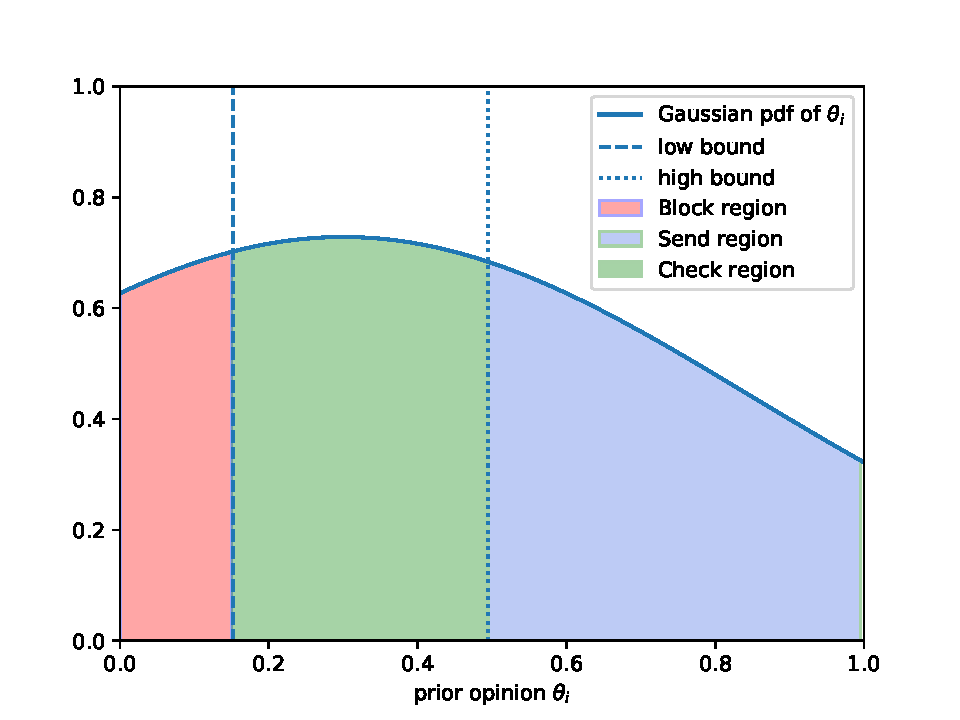
\includegraphics[width=.75\textwidth]{Figures/Zbounds.pdf}
	%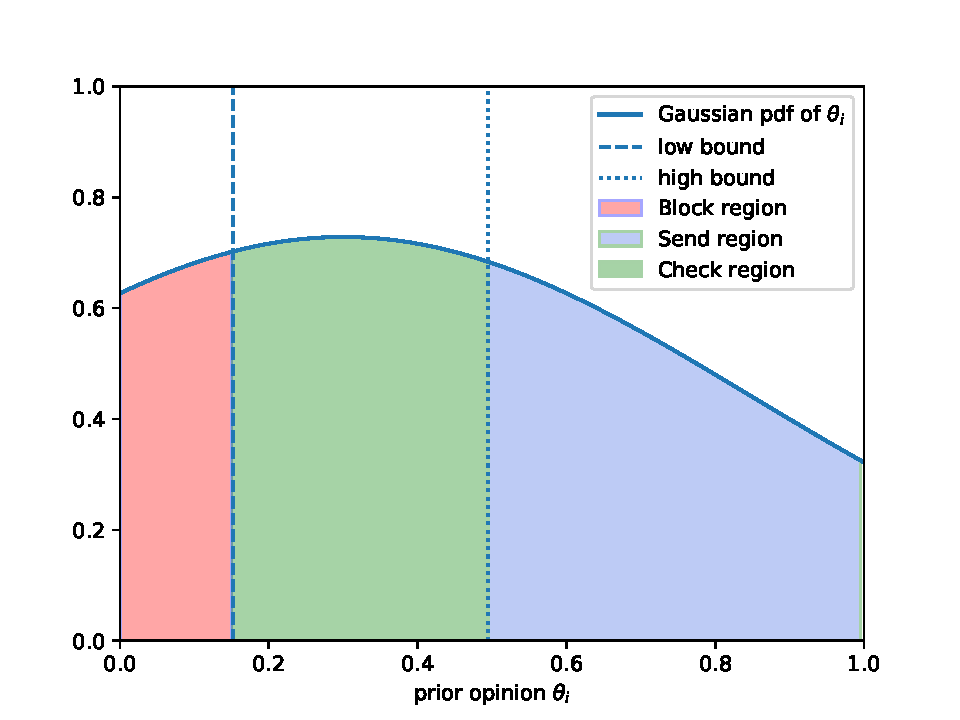
\includegraphics[width=.75\textwidth, height=.3\textheight]{Figures/Zbounds.pdf}
	
	\caption{Regions (areas according to high and low thresholds) that characterize agents actions for different prior opinions in first round. Parameters: $v=K=0.4$, $a=90\%$ and $\theta_i \sim \mathcal{N} (\mu=0.3,\sigma^2=0.09)$.}
	
	\label{fig:boundsandAreas}
\end{figure}

In figure ~\ref{fig:boundsandAreas}, we have a Gaussian pdf and the bounds $\underline{Z}, \overline{Z}$ in first round $t=0$. We have three cases where:

\begin{itemize}
	\item Priors $\theta_i$ that are picked below $\underline{Z}$, inside the red area, consists of users that prefer to block the sharing process without even inspecting it.
	\item The green area, that is between the thresholds $\underline{Z}, \overline{Z}$, consists of agents with prior opinions such that they are more likely to check the story in first round.
	\item The blue area, above $\overline{Z}$ threshold, belongs to agents with such prior opinions that they are going to share the message with no inspection.
\end{itemize}

Now we proceed, with the next proposition, by proving that those thresholds are non increasing in $t$ and also the difference $|\overline{Z}_{it} - \underline{Z}_{it}|$ is non increasing and non zero while $t \rightarrow \infty$.

\begin{prop}
	Given an agent $j$ and thresholds $\underline{Z}_{jt}$, $ \overline{Z}_{jt} \in (0,1)$, it holds that $\underline{Z}_{jt}$ and $ \overline{Z}_{jt}$ are decreasing in $t$ as well as the difference  $|\overline{Z}_{jt} - \underline{Z}_{jt}|_{t \rightarrow \infty}$
	\label{prop:decreasingZetas}
\end{prop}

\begin{proof}
	The claim is complete if we prove that $w_{it}$ is non increasing. That is obvious since $w_{it} = \displaystyle\prod_{k=0}^{t-1} \frac{S_{ik}}{S_{ik}+C_{ik}}$ is an product of quantities such that $ S_{it}, C_{it} \in (0,1)$, thus $w_{jt+1} < w_{jt}$, $\forall t$. For the difference $|\overline{Z}_{it} - \underline{Z}_{it}|$ let's assume that we have a agent $j$ with $\theta_j$, we compare the difference in round $t$ with the next round $t+1$. We have that:
	$$|\overline{Z}_{j(t+1)} - \underline{Z}_{j(t+1)}|-|\overline{Z}_{jt} - \underline{Z}_{jt}|=$$
	
	$$=
	\displaystyle\frac{1}{2\alpha-1}\left[\frac{\beta v w_{j(t+1)} (1-K)}{(1-v)K}-(1-\alpha)\right]-\displaystyle\frac{1}{2\alpha-1}\left[\frac{\beta v w_{j(t+1)} K}{(1-v)(1-K)}-(1-\alpha)\right]- $$
	
	$$\left\{
	\displaystyle\frac{1}{2\alpha-1}\left[\frac{\beta v w_{jt} (1-K)}{(1-v)K}-(1-\alpha)\right]-\displaystyle\frac{1}{2\alpha-1}\left[\frac{\beta v w_{jt} K}{(1-v)(1-K)}-(1-\alpha)\right]\right\}=$$
	
	$$\displaystyle\frac{1}{2\alpha-1} \left[ \frac{\beta v (1-K)}{(1-v)K} (w_{j(t+1)}-w_{jt}) -
	 \frac{\beta v K}{(1-v)(1-K)} (w_{j(t+1)}-w_{jt})\right]=
	$$
	
	$$ = \delta (w_{j(t+1)}-w_{jt})
	$$
	where $\delta$ is a constant such that $\delta>0$ for $K<0.5$ and $a>0.5$. Since $w_{j(t+1)}<w_{jt}$ we have that the difference is decreasing and it is non zero.
	
	The proof is equivalent using the assumption ~\ref{assum:AgentsPerceptionOfThetas} where $S_{it}$ and $C_{it}$ are replaced by $S_{it}^j$ and $C_{it}^j$ respectively, $\forall j \in path(root,i)$.
\end{proof}

With proposition ~\ref{prop:decreasingZetas}, we have the next important corollary for the sharing process, that expands the cascading behavior in ~\cite{papanastasiou} for sharing trees.

\begin{corollary}
	Let $G'$ be a sharing tree as specified in section ~\ref{sec:SharingProc}. There exists a certain depth $h_c$ at which the best response is to share without inspect. More specifically, there is a depth $h_c$ such that $\overline{Z}_{ih_c} \leq 0$ for some agent $i$ or equivalent, $h_c = min \left\{h \mid S_{ih}=1 \text{ or } \overline{Z}_{ih_c} \leq 0\right\}$.
\end{corollary}

\begin{figure}
	\definecolor {processblue}{cmyk}{0.96,0,0,0}
	\definecolor {processred}{cmyk}{0.96,0,0,0}
	\centering
	\tikzstyle{c} = [thick,draw, circle, minimum size=2,top color =white ,minimum size=2, bottom color = processblue!20,processblue]
	\begin{tikzpicture}[main/.style={c},
		level distance=15mm,
		level 1/.style={sibling distance=60mm},
		level 2/.style={sibling distance=30mm},
		level 3/.style={sibling distance=15mm},
		level 4/.style={sibling distance=12mm},
		end/.style = {draw, circle, minimum size=2,fill,top color=white,bottom color=red!20,red},
		critical/.style = {draw, circle, minimum size=2,fill,top color=white,bottom color=green!20,green}]
		\node (a)[main,label=left:{$\theta_1$}]{}[edge from parent]
		child {
			node (b) [end,label=left:{$\theta_2$}]{}
			child {node [main,label=left:{$\theta_4$}]{}
				child{ node  [main,label=left:{$\theta_8$}]{} }
				child{ node [main,label=left:{$\theta_9$}]{} }
			}
			child {node (c) [end,label=left:{$\theta_5$}]{}
				child{ node [main,label=left:{$\theta_{10}$}]{} }
				child{ node (d) [end,label=left:{$\theta_{11}$}]{}
						child{ node [main,label=left:{$\theta_{14}$}]{} }
						child{ node (k) [end,label=left:{$\theta_{15}$}]{} 
							child{ node (T) [critical,label=left:{$T_c$  $\theta_k$}] {} }
						}
				}
			}
		}
		child {node (e) [main,label=left:{$\theta_3$}]{} 
			child {node [main,label=left:{$\theta_6$}]{}
				child{ node [main,label=left:{$\theta_{12}$}]{} }
				child{ node [main,label=left:{$\theta_{13}$}]{} }
			}
			child {node [main,label=left:{$\theta_7$}]{}
			}		
		};
		\draw [->,color=red] (a) -- (b);
		\draw [->,color=red] (b) -- (c);
		\draw [->,color=red] (c) -- (d);
		\draw [->,color=red] (d) -- (k);
		\draw [->,color=green] (k) -- (T);
	\end{tikzpicture}
\caption{The critical round $T_c$ at where the best response of an agent in that depth is to share without inspecting an event.}
\label{fig:CriticalTime}
\end{figure}

Since each path expands as an independent experiment (agents know only how many of their predecessors shared), for each of these paths there is a certain depth that is critical. In the case of a path, where agents react in sequential manner, the round represents the number of agents that react. In other words, we have a critical agent positioned in a specific spot of the path such that, after a certain amount of reactions, at round $T_c$ the best response of $T_c + 1$ agent is to send without inspecting the story. In figure ~\ref{fig:CriticalTime} we have an example of a sharing process alongside with the propagation network. The sequence of agents $\left\{ \theta_1, \theta_2, \theta_5, \theta_{11}, \theta_15  \right\}$ reached in such depth that the quantity $w_{kT_c}$ will affect agents' belief that the story is fake, $q_{kT_c}$ that the expected response is to share the story without inspection. In other words, agents' interpretation of their depth is an increasing possibility of an existing agent that checked the story and decided to share to the subsequent agents.

One question that emerges from the above analysis is the impact of depth over agents opinion that a story is false, namely $q_{it}$.

\begin{corollary}
	For an agent $i$ with prior opinion $\theta$ and his posterior belief that $m=y$ is fake, $q_{it}$, it holds that:
	\begin{itemize}
		\item If agent $i$ chooses action $S$ in round $t_0$, $A_{it_0} = S$ then $\forall t>t_0$ subsequent rounds, $A_{it}=S$.
		\item If agent $i$ chooses action $B$ in round $t_0$, $A_{it_0} = B$ then $\forall t \in [1,t_0]$ previous rounds, $A_{it}=B$.
	\end{itemize}
	\label{cor:SBBOUNDS}
\end{corollary}

\begin{proof}
	We will prove the first bullet, since the second is proven in symmetrical manner with opposite monotonicity. Lets assume that agent chooses to share a story without inspecting it, at a given time $t_0$ which means that $A_{it_0}=S$. This choice optimal when his expected utility is maximized via action $S$, more specifically, whenever it holds that $1-q_{it_0}>q_{it_0}$ and $1-q_{it_0}>1-K$. Since $q_{it}$ is decreasing in time, then the quantity $1-q_{it_0}$ is increasing in time and since it is upper bound for both $q_{it}$ and $1-K$, then it will remain an upper bound as $t$ increases, which proves the claim. For the second bullet, the proof is symmetric since $q_{it_0}>1-q_{it_0}$ and $q_{it_0}>1-K$ when the response is $A_{it_0}=B$. Adding the fact that $q_{it}$ is decreasing in time, from lemma ~\ref{lemma:monotontime}, we have that the above inequalities hold, for each round $1<t<t_0$.
\end{proof}

 %agents		 	 ch:3
\chapter{Platforms' Inspection Mechanisms}
\label{ch:Platforms Problem}

So far we created a setup for information exchange between a group of rational agents alongside with the rationalization of the assumptions we made for our model. The next step is to define the behaviour of our authoritative entity, in our case the platform which is the social medium where agents interact and share stories with each other. Given that the platform has an overview of the whole process, we utilize this knowledge under a number of assumptions, to develop appropriate tools for our platform in order to intervene and inspect information. Our goal is to consider the properties of our network that will specify the optimal time for inspection. 

In this chapter we introduce platform's role in the sharing process model and the inspection problem. We modify the basic sequential model introduced by ~\cite{papanastasiou} in order to work for asynchronous propagation within tree structures, adding the necessary assumptions.  We continue with an analysis of the properties that emerge from those assumptions. Finally, we leverage the structure features in order to find an approximate solution for intervention and inspection of a story at proper time. 

\section{Introducing Platform in the Sharing Process}
\label{sec:platformIntro}

So far we have an ecosystem where agents share messages called \textit{stories}, as we mentioned in previous chapter, and their actions are under the assumption that are responsible individuals. This technically means that they act in order to maximize their expected utility by not sharing non trusted stories according to their judgment. Now we introduce the platform, where those individuals reside in. Examples of such entities are Facebook, Twitter, YouTube and many more, where millions of user interact and share information with each other. In our case study, platform is a \textit{super} agent providing those online services in order for agents to interact with each other. In our study, the platform observes the evolution of the propagation tree, and infers the posterior probabilities of the involved users, so as to have its own posterior belief about the validity of a story.

\begin{figure}[t]
	\centering
	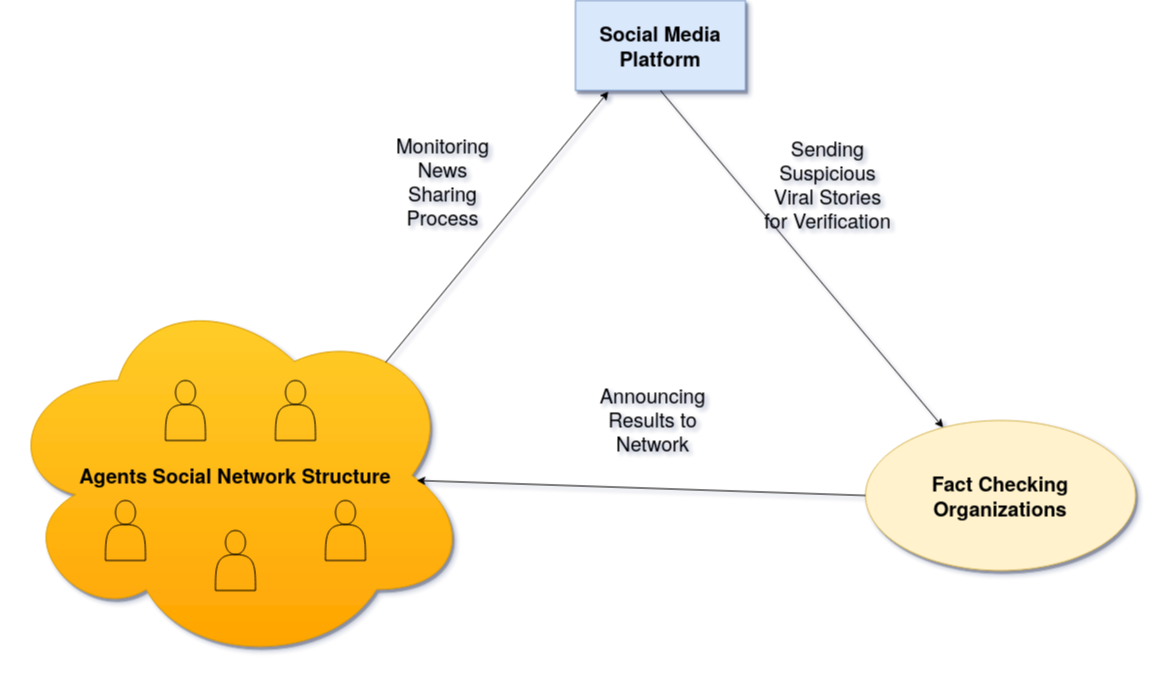
\includegraphics[width=.75\textwidth]{Figures/EntityDiagram.png}
	%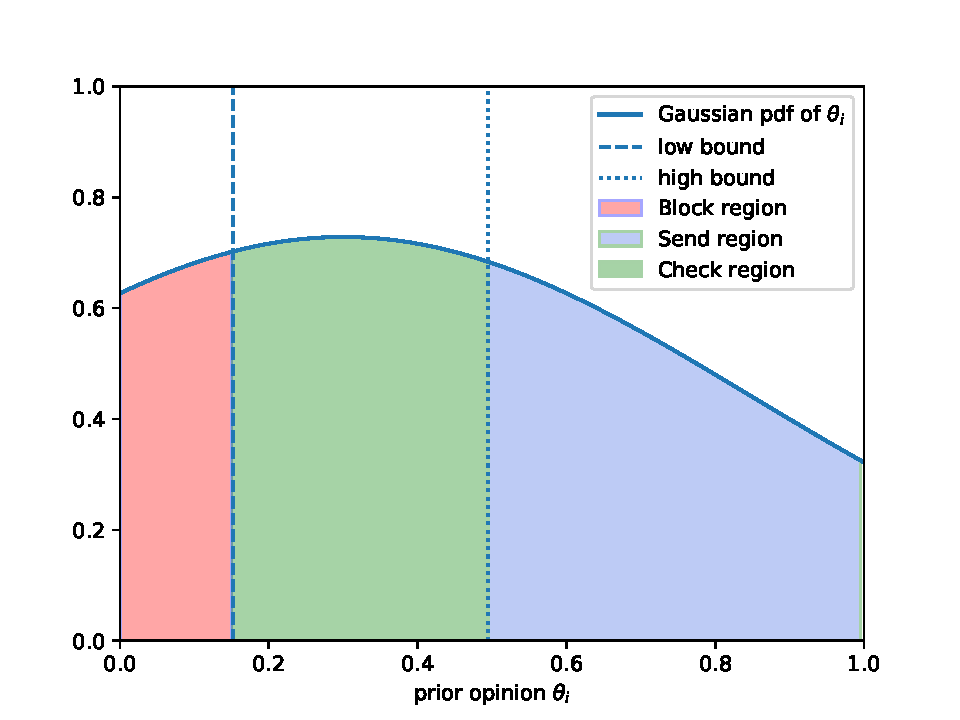
\includegraphics[width=.75\textwidth, height=.3\textheight]{Figures/Zbounds.pdf}
	
	\caption{The fact checking model of a social media service. The fact-checking process is assumed to an external service for the platform, which of course comes with a given cost for the platform. In practical scenarios, the platforms cannot conduct a fact check over stories because this would affect their policy, given that fact checking comes with a cost.}
	
	\label{fig:entityDiagram}
\end{figure}

In figure ~\ref{fig:entityDiagram} we have our ecosystem with the introduction of platform. We see that our platform monitors the activity of agents network in order to maintain a trustworthy social network of information sharing. If platform suspects that a story is shared effortless (without any inspection), then there is a global check via fact checking organizations. Afterwards, the results are announced to our network and there are two options:

\begin{itemize}
	\item If the story is validated as truthful, then this announcement leads to a sharing cascade. Additionally, the platform will receive a discounted reward for each share of the story in our network.
	\item If the story is fake, then the sharing process is terminated and the the platform will receive only a penalty for each (previous) share of the fake story, along with a fixed global-check cost. 
\end{itemize}
In our case study, we assume that the inspection yields a perfect result. This assumption holds for both agents and the authoritative entities such as the platform or fact checking partners. We also remind that this setup is easily extensible for cases where the fact checking action occurs with error. 

Another important part of our setup is the amount of privileges that such a platform possesses. We mentioned above that our platform is a super user with extra knowledge. We assume that our platform observes the creation of edges in our network without knowing if they are product of checking action or blindly sharing the story. In other words, platform observes reactions at given round $t$ from agents without knowing the exact action, i.e. if it $A_{it}=S$ or $A_{it}=C$ in round $t$. Additionally, the platform is unaware if an agent discontinued the sharing process by blocking of checking the story. More specifically, platform cannot observe the round $t$ where an agent decided to not share a story with either $A_{it}=B$ or via checking with $A_{it}=C$. This assumption reflects a real life application where a social media administrator cannot monitor if an individual user of such a service conducted a research or not in order to share information within a network. 

This brings us to a stronger assumption that makes the building block of our model.

\begin{assumption}
	The exact value of random variables $\theta_i \sim \mathcal{N} (\theta,\sigma^2)$ for each agent $i$ are hidden from platform. Platform only assumes a normal distribution $N(\theta,\sigma^2)$ for the independent sampling of prior beliefs for the agents.
\end{assumption}
The reasoning behind this assumption, that strengthens our model in order to work under uncertainty, is that we cannot predict the exact value of a prior opinion of a random agent. For example, let's assume that we have an emerging topic. In such case, most probably, we do not have prior opinions formed on the topic or even worse, we formed wrong prior opinions. Another important property this assumption has is the fact that this model is more confidential since we can work without monitoring users of such services where there are issues of private information leaks.

As we mentioned above, the platform monitors reactions of agents, more specifically, those reactions that share information from parents to children. In other words, platform increases the round from $t$ to $t+1$ whenever a node $i$ decides to share and create edges to his \textit{friends}, \textit{followers} or children (from data structure perspective). We need to decide how those agents are picked to react and choose an action at round $t$. There are two approaches for that issue:

\begin{itemize}
	\item Agents that are terminal leaves in the sharing tree are picked uniformly at random.
	\item Agents are picked with probability $(1/m)^l$ where $m$ is the amount of children that each node have (for $m$-ary trees) and $l$ is the height of node $i$ in the sharing tree.
\end{itemize}

\begin{figure}
	\definecolor {processblue}{cmyk}{0.96,0,0,0}
	\definecolor {processred}{cmyk}{0.96,0,0,0}
	\tikzstyle{c} = [thick,draw, circle, minimum size=2,top color =white ,minimum size=2, bottom color = processblue!20,processblue]
	\centering
	\begin{tikzpicture}[main/.style={c},
	level distance=15mm,
	level 1/.style={sibling distance=20mm},
	level 2/.style={sibling distance=30mm},
	level 3/.style={sibling distance=15mm},
	end/.style = {draw, circle, minimum size=2,fill,top color=white,bottom color=red!20,red},
	discovered/.style = {draw, circle, minimum size=2,fill,color = red},itria/.style={
		draw,shape border uses incircle,
		isosceles triangle,shape border rotate=90,yshift=-1.45cm}]
	\node (a)[main,label=left:{$\theta_1$}]{}[edge from parent]
	child {
		node (b) [end,label=left:{$\theta_2$}]{}
			child {
				node (t) [itria]{L}
			}
	}
	child {
		node (c)[main,label=left:{$\theta_3$}]{} 
	}
	child {
		node (d)[main,label=left:{$\theta_4$}]{} 
	};
	\draw (a) -- (b) node [->] {};
	\draw (a) -- (c) node [->] {};
	\draw (a) -- (d) node [->] {};
	\end{tikzpicture}
	\caption{An example of a ternary sharing tree where each agent is picked uniformly at random to react. The right triangle $L$ is a subtree of the sharing tree.}
	\label{fig:unbalancedCase}
\end{figure}

It is obvious that the first approach tends to create unbalanced trees in depth first manner. In figure ~\ref{fig:unbalancedCase} we see such a case. After the root decided to share the information, let's assume that node $\theta_2$ is picked with probability $1/3$, since we have a ternary propagation tree, tree, to react at round $2$. The set of leaves at that round, we call it frontier from now on, consists of nodes $\theta_3$, $\theta_4$ and the children of $\theta_2$, $D_{\theta_2}$. Because we assumed that agents are picked uniformly at random, hence the probability of picking a node on the frontier is now $1/(\mid \{\theta_3,\theta_4\} \cup D_{\theta_2}) \mid$, in case of our example it is $1/5$ since we have $3$ children of $\theta_2$ plus the nodes in level $1$. This implies that $\theta_2$ will probably will be picked, with probability $3/5$, rather than $\theta_3$ or $\theta_4$, with probability $2/5$. Moving forward in the next round, the probability of picking one node to react in the subtree $L$ will increase once again, making more likely an expansion of the sharing tree towards $L$.

On the other hand we have the second approach where the level of each node matters, hence we have that node $i$ is picked with probability $(1/m)^l$ where $m$ is the amount of children each node is assumed to have\footnote{We are using mean field analysis in our approach with an average degree for children in our tree structure. Thus we are developing this model over $m$-ary trees.} and $l$ is the level where node $i$ belongs. This approach is used to tackle down the issue that we have with unbalanced tree when we are picking uniformly at random and also it is reasonable to say that we expect from nodes who received the story earlier to react faster than freshly activated nodes in the sharing tree.

Now that have established the role of the platform, alongside with the appropriate assumptions, we proceed with the technical part and the introduction of the optimal inspection problem. 


\section{Platforms' Inspection Problem}
\label{sec:platformInspection}

Since we assumed that inspection yields a perfect outcome, it is sufficient to find one agent that inspected the element. If an agent that inspects the story and decides to share that means he found the story truthful. Because we assumed that the result is irrefutable, the announcement of that the story is truthful will trigger an information cascade in the sharing tree, and each sharing action afterwards will increase the discounted reward that platform receives, i.e. advertise revenue or another monetization strategy that is benefit from sharing content. Apart from the agents' private inspections (fact-checks) for the type of a story, the platform may also intervene by requesting a global fact-check (e.g., from an external third-party fact-checking service) and then communicating the result of this inspection to the entire community.  

On the other hand, we have agents that are not reacting, and we cannot presume if the chose $A_{it} = C$ or $B$ as an action, as we specified in section ~\ref{sec:platformIntro}. An agent might block a story either with or without inspection and that is hidden from platform since it does not posses the exact value of $\theta$ for each agent nor it is clear if the agent inspected or plainly blocked the story. Thus it is important for the platform to estimate the probability that some agent received the story and decided to inspect and block it. Once again, this event is sufficient enough since inspection is perfect. The platform can also utilize the probability of that event and dispute the validity of that story via fact checking organizations. We assume that the intervention of the platform in the evolution of the emergent story via fact-checking comes with a cost $K_p$. Now that we established those two warning mechanisms for global check, we provide two propositions in order to calculate the probabilities of those events.

\begin{prop}
	Let $T$ be a sharing tree and $m=y$ is the story that propagates in $T$. Then the platform's belief there exist an agent $i$ and $A_{it}=C$ at some round $t$ in $T$, under the assumption that platform observes independent random experiments over agents, is: 
	$$r_T = 1-\mathbb{P}_{pT} \{\forall i \in \mathcal{V}_{T}: A_{it}=S \mid H_i,m=y \} =  1 - \displaystyle \prod\limits_{\substack{k = 0 \\ i \in \mathcal{V}_{T}}}^{t-1} \mathbb{P} [A_{ik} = S_{ik}^p] $$ where $\mathcal{V}_{T}$ are the set of nodes of $T$, respectively.
	\label{prop:GreenProb}
\end{prop}

Before we begin with the proof of proposition ~\ref{prop:GreenProb}, it is important to mention that time is irrelevant in that equation since we can rearrange the sequence of shares and agents id's in order. We keep the annotation of $A_{it}$ though to avoid \textit{polluting} this thesis with unnecessary notations. That being said, we only use the next definition in order to specify the platform's belief over agents' $i$ action:

\begin{definition}
	For each action $A_{it} = \{B,C,S \}$ of an agent $i$ in round $t$, we define the probabilities $B_{it}^p$, $C_{it}^p$ , $S_{it}^p$ that estimate the platform's perception over the probabilities $B_{it}$, $C_{it}$ , $S_{it}$ for each action respectively.
\end{definition}

\begin{proof}{(Proposition ~\ref{prop:GreenProb})}
	We need to calculate the probability of the event that at least one agent chose C given that we have a sharing $T$ and a story claiming $m=y$. Let this probability be $r_T$. We have that $ r_T=\mathbb{P}_{pT} \{\exists i \in \mathcal{V}_{T}: A_{it}=C \mid T,m=y \} = 1-\mathbb{P}_{pT} \{\forall i \in \mathcal{V}_{T}: A_{it}=S \mid T,m=y \}$. The last equality is equivalent, since the worst case scenario is that none inspected the story and chose to share, in other words $A_{it}=S$, $\forall i \in  \mathcal{V}_{T}$. Since we assumed that events are independent the probability $r_T$ is the product of all those independent experiments, thus $ r_T = 1-\mathbb{P}_{pT} \{\forall i \in \mathcal{V}_{T}: A_{it}=S \mid T,m=y \} \approx 1 - S_{00}^p S_{11}^p S_{22}^p . . .S_{i(t-1)}^p$ where we rearranged agents id's to match the round at where they reacted throughout the propagation process due to the fact that actions are calculated independently. Thus we have that $r_T =  1 - \displaystyle \prod\limits_{\substack{k = 0 \\ i \in \mathcal{V}_{T}}}^{t-1} \mathbb{P} [A_{ik} = S_{ik}^p]$, where $S_{ik}^p$ is platform's perceived value that agent $i$ chose $S$ in round $t$. 
\end{proof}
This value is the platform's posterior belief, just before the $t$-th round of sharing, that at least one of the internal nodes actually conducted a check. Additionally, the above calculation provides us with a warning indicator that approximates the approach followed in ~\cite{papanastasiou}, where platform has a normalized belief $q_p$ that a story is fake, based on the evolution of a sharing process in a path. This approach cannot be used in the case where we have a tree structure since there are nodes that we are unsure of their reaction. To further understand this issue, let's assume that we have an $m$-ary tree and there is a node in first level that did not react after $m+t_0$ rounds. If the value of $t_0$ is large enough at a point where the process evolved in lower depths, then it is safe to assume that agent $i$ either rejected the story by choosing $B$ or inspected the story and disclosed it's validity with $C$. It is obvious that there is a challenge in order to calculate this probability since we need to take into account the fact that the agent's reaction concerning shares are partially hidden. The next proposition calculates the existence of such an agent, more specifically, the probability that at least one agent inspected the story and found it fake.

\begin{prop}
	Let $T$ be an $k$-ary sharing tree and $m=y$ is the story that propagates in $T$. Then the platform's belief that a terminal node $i$ blocked the story $m$ by inspecting it, $A_{it}=C$, in round $t$ is:
	$$ n_{it} =  [1-(1/k)^{l_i}]^{t-t_i} (1/k)^{l_i} \frac{C_{it}^p}{B_{it}^p+C_{it}^p}$$
	where $l_i$ is the level of node $i$ in $T$ and $t_i$ is the round where $i$ received the story.
\end{prop}

\begin{proof}
	Let $i$ be a random node of $T$ and $l_i > 0$ \footnote{We do not bother proving the proposition for root since it holds trivially.} its' depth in it. We will prove the claim by induction over $t-t_i$. For $t-t_i = 0$, which means after the first time that node $i$ was candidate to react, there are to cases:
	\begin{itemize}
		\item With probability $1-(1/k)^{l_i}$, node $i$ it is not picked to react at current round.
		\item With probability $(1/k)^{l_i}$, node $i$ reacts in that round.
	\end{itemize} 
In case where the node is picked to react, the probability that this node will inspect the story and then decide to block it because it is fake, is equal to $\frac{C_{it}^p}{B_{it}^p+C_{it}^p}$. Thus we have that: $$n_{i,t_i} = (1/k)^{l_i} \frac{C_{it}^p}{B_{it}^p+C_{it}^p}$$
after the first round that $i$ was candidate to react and it was picked for that round. On the other hand, if we move at the next round where $i$ is once again candidate to react, then the probability that he will react in $t-t_i = 1$ is: $$n_{i,t_i+1} = P\{\text{did not react in previous round\} P\{ \text{reacts in t round with C}\}} = $$
$$[1-(1/k)^{l_i}] (1/k)^{l_i} \frac{C_{it}^p}{B_{it}^p+C_{it}^p}$$ Assuming the claim holds for $t-t_i$, we can easily prove that it holds for $t-t_i+1$ as well.
\end{proof}

\section{Optimization Criterion for Inspection Time}
\label{sec:optimize}

In this section we develop an optimization criterion based on utility maximizing approach as in \cite{papanastasiou}. Recall that we developed a model where the agents are socially responsible, which means that they share only truthful stories and also aim to maximize their utility. We assume that it is to the interest of the platform to forbid the propagation of fake stories, i.e. such platforms try to maintain their reliability in order to form a profitable model from advertisement revenue. In each round $t$, the platform observes an activation of a node in the sharing tree. This means that rounds represent a counter for the amount of nodes that reacted throughout the sharing process. At each round, and according it's belief for the validity of the story, platform can perform a global check if it suspects that the story is fake and can cause damage to it's credibility. In case where platform believes that the story is truthful we do not have any interruption of the story. 

In order to develop a criterion to calculated the existence of an optimal time to interrupt the process in order to avoid further damage that un checked shares will cause, we develop a utility maximizing scheme. We assume that if the story is fake, then for each successful share platform receives penalty $P$. For each successful share of a truthful story, the platform will receive a discounted reward $R$, with a discount factor $\delta < 1$ that is affected by the depth of the sharing process. The discount factor rationalization is that freshly shares are more relevant in order to form an opinion over the validity of our story. If platform decides to intervene in order to check the validity of a story, this action occurs with a cost $K_p$, and the this decision is once and for all. This means that after the announcement of the results, we have two cases. If the current story is fake, then the process ends with the appropriate penalties for each share, while if it is truthful, an information cascade triggers and platform will collect all future discounted rewards. 

Platform determines its' policy by estimating the utility of the sharing tree and the option of inspecting or not is viable respectively. At each round $t$, the process already created a sharing tree $T$. Therefore, we have an \textit{observed} utility that either we will receive penalty if the story is fake or collect reward otherwise. We define the utility that platform gains, for each agent $i$ in round $t$, as:

\begin{equation}
g_{pT} (V) = 
\begin{cases}
P, & \text{w.p. } S_{it}q_{pT} \textit{ if } V=F \\
R, & \text{w.p. } (S_{it}+C_{it})q_{pT} \textit{ if } V=T\\
0, & \text{else} \\
\end{cases}
\label{eq:platUtility}
\end{equation}

Assuming that platforms belief, that the story is fake, is $q_{pT}$, we have the following lemma for the observed utility of our platform:

\begin{lemma}
	The expected observed discounted utility that platform gains from a sharing tree $T$ is:
	$$ O_{p}(T) = \sum_{i \in \mathcal{V}_{T}}  \delta^{l_i} \left[ P ( S_{it}^p q_{pT} ) + R ( S_{it}^p+C_{it}^p)q_{pT}  \right]$$ where $l_i$ is the depth that agent $i$ belongs and $\mathcal{V}_{T}$ is the set of nodes/agents that belong in $T$.
\end{lemma} 

\begin{proof}
	Similarly to proposition ~\ref{prop:ExpUtility}, we have that:
	$$ O_{p}(T) =  \mathbb{E} [g_{pT} (V)]_{\forall i \in \mathcal{V}_{T}, V \in \{T,F \}}  $$
	Thus, for each internal node that we already observed its reaction, we receive a discounted reward in case it successfully shared the story. In case an internal node shares a fake story, and assuming platform's belief that the story is fake equals to $q_{pT}$, it comes with penalty $P$. According to equation ~\ref{eq:platUtility}:
	$$ O_{p}(T) =  \mathbb{E} [g_{pT} (V)]_{\forall i \in \mathcal{V}_{T}, V \in \{T,F \}} = \sum_{i \in \mathcal{V}_{T}}  \delta^{l_i} \left[ p ( S_{it}^p q_{pT} ) + r ( S_{it}^p+C_{it}^p)q_{pT}  \right]$$
	 
\end{proof}

Let's assume that we observe a sharing tree $T$ and define the frontier $\mathcal{F}$, that is a subgraph of $T$, as those nodes that are leaves of $T$ (candidates to react). Then we can calculate the expected utility that we will gain with the addition/s of nodes that belong in frontier. Let's assume that node $j$ will react and enter in the sharing tree such $T \cup \{j\}$. In worst case scenario, where the story is fake, we expect from the same tree, a penalty for each descendant of $j$. We have two possible policies, to make a global check, annotated as $\mathcal{C}$, and collect reward/penalty or to let the process continue, annotated as $\mathcal{E}$, and reevaluate the expected utility once again. If the platforms' belief that the story is fake equals to $q_{pT}$ then the expected discounted utility gained from subtree $T'$ if platform chooses to global check, is: 
$$ (\delta^{l_i} R + \delta^{l_i+1} k R + \delta^{l_i+2} k^2 R+...) (1-q_{pT}) - K_p $$
where $K_p$ is the negative utility gained because the cost of inspection. If $\delta k <1 $ we conclude that:
$$ U_{\mathcal{C}} =\delta^{l_i} (R+ \delta k R+\delta^2 k^2 R+...)(1-q_{pT}) - K_p = \delta^{l_i}(1-q_{pT}) \frac{R}{1-\delta k}-K_p$$
Observe that this is the anticipated utility gained only by one agent $j \in \mathcal{F}$. If we want to in account every other agent $j$ in frontier we sum up the anticipated costs and we have:

$$ U_{\mathcal{C}} = \sum_{j \in \mathcal{F}} \delta^{l_j+t}(1-q_{pT}) \frac{R}{1-\delta k}-K_p$$

Now let us discuss the utility that the platform will receive if it decides that it will not intercept the sharing process. According to that strategy, $\mathcal{E}$, we have the next probable outcomes:

\begin{itemize}
	\item With probability $C_{it}$, agent $i$ checks and decide to only share a truthful story and platform collects reward.
	\item With probability $(1-q_{pT}) S_{it}$, agent $i$ shares a truthful story and platform collects reward.
	\item With probability $q_{pT} S_{it}$, agent $i$ shares a fake story and platform receives penalty.
\end{itemize}

Then, the utility we gain from agent $i$, if the platform decides to $\mathcal{E}$, is given by the equation bellow:
$$C_{it}(1-q_{pt})R + S_{it}(1-q_{pT})R + S_{it} q_{pT} P$$
Observe that the reaction of agent $i$ creates a subtree $T'$ with node $i$ as root. Then we have the recursive formula for the discounted anticipated utility that will grow exponentially and make the calculations complex. It is obvious that it is not feasible to calculate the utility that way for two main reasons. First reason is the complexity of calculations and the fact that is hard to find a closed form type for that expected utility in order to maximize it. Secondly, the platform's belief is changing while the depth increases and this formula should recalculate $q_{pT} $ at each step which increases the complexity even more.

In order to deal with that problem, we propose the next approximation method. Suppose that platform decided already the validity of the story at round $t$. Then we have two probable cases where:

\begin{itemize}
	\item The story is fake with probability $q_{pT}$ and platform chooses strategy $\mathcal{E}$.
	\item The story is true, following the same strategy.
\end{itemize}
This modification simplifies the calculations by breaking down the problem in two different cases. Let us see what happens in the case where platform decides that the story is fake. There is  only one way that fake stories will propagate after the platform decides to let the propagation evolve and it is only if an agent decides to share without check, namely $S_{ih}$. Notice that if he decided to check the story given that platform believes it is fake, implies that the agent will discontinue the propagation. So we have that the utility in that case is:
$$ \sum_{t=0}^\infty \delta^{l_j+t} \left[ S_{l_j+t} k^t P \right] $$
where $l_j$ is the depth that agent $j$ belongs, $\mathcal{T}_j$ is the subtree, rooted on agent $j$ that belongs in frontier and $\delta$ is the discount factor. If the platform decides that a story is true over a propagation tree $T$, then the story propagates with two ways. A story can be sent to the next level in the tree with $S$ or $C$ action since it is true and agents even when fact-checking it, will share it. Therefore, the probability that a story is shared equals to $(1-B_{it})$. This observation simplifies things since it is easier to express the monotonicity of the expression bellow. For that policy, we have that the next equation that expresses that utility:

$$ U_t^A = \sum_{t=0}^\infty \delta^{l_j+t} \left[ (1-B_{l_j+t}) k^t R  \right]$$where $\mathcal{T}_j$ is the subtree, rooted on agent $j$ that belongs in frontier.
Now we are ready to collect those expressions in the next proposition that gives a formula for the platforms utility if it lets the propagation evolve.


\begin{prop}
	The anticipated utility that platform gains if it decided to let the news sharing process evolve, for an agent $ j \in \mathcal{F}$ in frontier is:
	
	$$ U_f^A = \sum_{t=0}^\infty \delta^{l_j+t} \left[ S_{l_j+t} k^t P \right] $$for fake stories and
	 $$ U_t^A =\sum_{t=0}^\infty \delta^{l_j+t} \left[ (1-B_{l_j+t}) k^t R  \right]$$for truthful.
\end{prop} 
Both of the above values will express the utility the platform gains for each agent for a sub-tree created in the frontier, rooted at agent $j$. This means we get the appropriate utility from agent $j$, discounted by $\delta^{l_j}$, plus the corresponding discounted utility of his $k$ descendants and so on. Before we find the boundaries, we collect the above quantities in order to form the final expression of the platforms expected discounted utility:
$$ U_p = O_p (T) + A_p (T)$$
where the anticipated utility of our propagation tree network $T$ is:


\begin{equation}
U_p(T) = 
\begin{cases}
 &  O_p (T)+U_{\mathcal{C}}(T) \text{ , Global-check } \mathcal{C}\\
 &  O_p (T)+U_{\mathcal{E}}(T) \text{ , Let-evolve } \mathcal{E}\\
\end{cases}
\label{eq:utilsPlat}
\end{equation}


Now remains the issue of limits. As it was previously mentioned, for each agent in the frontier, in order to calculate the anticipated utility we have to calculate the probabilities of $S$ and $B$ indefinitely. In order to deal with that, we need convergence for $U_f^A$ and $U_t^A$. The next proposition uses the monotinicity of probabilities $S$ and $B$ in order to bound those values.

\begin{prop}
	For the anticipated utilities over fake and truthful news respectively, it holds that:
	$$ U_f^A  < \delta^{l_j} S_{l_j} \frac{P}{1-\delta k} = \overline{U}_f^A$$for fake stories and
	$$ \delta^{l_j}(1-B_{l_j}) \frac{R}{1-\delta k} = \underline{U}_t^A < U_t^A  $$for truthful, where $j$ is the corresponding root agent that belongs in frontier.
	\label{prop:firstThresholds}
\end{prop}

\begin{proof}
	We have from corollary ~\ref{cor:SBBOUNDS} that $S_{l_j}$ probability is increasing in depth ${l_j}$, thus we have that $(S_{l_j} < S_{l_i}$ in every level $l_i$ lower than $l_j$. Thus we have that:
	
	$$ U_f^A = \delta^{l_j} (P S_{(l_j)} + \delta k PS_{(l_j + 1)} +\delta^2 k^2 P S_{(l_j + 2)}+...) < $$ $$ \delta^{l_j} (P S_{(l_j)} + \delta k PS_{(l_j)}+\delta^2 k^2 P S_{j(l_j)}+...) = \delta^{l_j}S_{l_j} \frac{P}{1-\delta k}$$when $P<0$
	
	Respectively, we have that $B$ is decreasing in depth. Thus $(1-B_{l_i}) > (1-B_{l_j})$ for every level $l_j$ lower than $l_i$. In similar manner we can restrict, the anticipated utility for the case a true story, such that:
	
	$$U_t^A = \delta^{l_j} (R (1-B_{(l_j)}) + \delta k R (1-B_{j(l_j + 1)}) +\delta^2 k^2 R (1-B_{(l_j + 2)})+...) > $$ $$ \delta^{l_j} (R (1-B_{(l_j)}) + \delta k R(1-B_{(l_j)}) +\delta^2 k^2 R (1-B_{j(l_j)}) +...) = \delta^{l_j}(1-B_{l_j}) \frac{R}{1-\delta k} $$ 	
\end{proof}
In the last proposition, we use the probabilities of root $j$ in the frontier, in order to bound the geometric series. This is an important step, which will help in advance to find a closed type equation for the anticipated utility. This allows the platform to make a better prediction instead of letting the process continue up to the point that agents propagation process arrive at some depth $T_c$ where they all choose to share.

\iffalse
The next proposition calculates upper and lower thresholds for the values $U_f^A$ and $U_t^A$ respectively. Those values and their existence depends on the starting state of the process and the perceived values of proposition ~\ref{prop:ZBounds}. Additionally, those bounds reduce the complexity of the calculations, since we do not go further in each subtree, in order to calculate the probabilities $B_{it},C_{it},S_{it}$.

\begin{prop}
	Depending on the initial state of thresholds of proposition ~\ref{prop:ZBounds}, it holds that:
	$$\underline{U}_f^A < U_f^A  < \overline{U}_f^A =  \delta^{l_j}B_{l_j} \frac{P}{1-\delta k}$$for fake stories and
	$$ \delta^{l_j}(1-S_{l_j}) \frac{R}{1-\delta k} =\underline{U}_t^A < U_t^A <  \overline{U}_t^A$$for truthful.
The above thresholds hold only when $S_{i0} > B_{i0}$ at the initial state.
	
\end{prop}


\begin{proof}
	\[
\delta^{l_j} B_{l_j} / (1 - k\delta) 
< \delta^{l_j} S_{l_j} / (1 - k\delta)
\Leftrightarrow
\delta^{l_j} P B_{l_j} / (1 - k\delta) 
> \delta^{l_j} P S_{l_j} / (1 - k\delta)
\]
	
The proof of this claim is similar with the proposition ~\ref{prop:firstThresholds}. We we only bound the values $(1-S_{l_i})$ and $(1-B_{l_i})$ with the constraint we have in the proposition that $S_{i0} > B_{i0}$ and the limits of geometric series are derived with the same manner. First, we have that initial $S_{i0} > B_{i0}$, thus we have that $1-S_{i0} < 1-B_{i0}$. From the monotonicity of those probabilities we have that:
\begin{align}
\begin{split}
1-S_{i1} < 1-B_{i1} \\
1-S_{i2} < 1-B_{i2} \\
... \\
1-S_{ih} < 1-B_{ih}
\end{split}
\end{align}
This proves the claim since we can bound all the terms from each inequality, such that:	
$$U_f^A = \delta^{l_j} (P S_{(l_j)} + \delta k PS_{(l_j + 1)} +\delta^2 k^2 P S_{(l_j + 2)}+...) >  $$ $$\delta^{l_j} (P B_{(l_j)} + \delta k PB_{(l_j + 1)} +\delta^2 k^2 P B_{(l_j + 2)}+...) >$$
$$\delta^{l_j} (P B_{(0)} + \delta k PB_{(0)} +\delta^2 k^2 P B_{(0)}+...) = \delta^{l_j}B_{0} \frac{P}{1-\delta k} $$
and
$$U_t^A = \delta^{l_j} (R (1-B_{(l_j)}) + \delta k R (1-B_{j(l_j + 1)}) +\delta^2 k^2 R (1-B_{(l_j + 2)})+...) >  $$ $$\delta^{l_j} (R (1-S_{(l_j)}) + \delta k R (1-S_{(l_j + 1)}) +\delta^2 k^2 R (1-S_{(l_j + 2)})+...)	>$$
$$\delta^{l_j} (R (1-S_{(l_j)}) + \delta k R (1-S_{(l_j)}) +\delta^2 k^2 R (1-S_{(l_j)})+...) = \delta^{l_j}(1-S_{l_j}) \frac{R}{1-\delta k}	$$
\end{proof}



Notice that the above boundaries are not that tight in terms of how they enclose the actual values. They also depend on the initial state of the system which is not necessary useful from algorithmic perspective. Their significance is on the time complexity and the fact that include all the characteristics of the propagation process, the discount factor, the platforms belief, the depth of the tree and the breadth (the average neighborhood size which is $k$).
\fi
\begin{figure}
	\definecolor {processblue}{cmyk}{0.96,0,0,0}
	\definecolor {processred}{cmyk}{0.96,0,0,0}
	\tikzstyle{c} = [thick,draw, circle, minimum size=2,top color =white ,minimum size=2, bottom color = processblue!20,processblue]
	\centering
	\begin{tikzpicture}[main/.style={c},
	level distance=15mm,
	level 1/.style={sibling distance=20mm},
	level 2/.style={sibling distance=30mm},
	level 3/.style={sibling distance=15mm},
	end/.style = {draw, circle, minimum size=2,fill,top color=white,bottom color=red!20,red},
	discovered/.style = {draw, circle, minimum size=2,fill,color = red},itria/.style={
		draw,shape border uses incircle,
		isosceles triangle,shape border rotate=90,yshift=-1.45cm}]
	\node (a)[main,label=left:{$\theta_1$}]{}[edge from parent]
	child {
		node (b) [main,label=left:{$\theta_2$}]{}
		child {
			node (t) [itria]{$T_1$}
		}
	}
	child {
		node (c)[main,label=left:{$\theta_3$}]{} 
		child {
			node (t) [itria]{$T_2$}
		}
	};
	\draw (a) -- (b) node [->] {};
	\draw (a) -- (c) node [->] {};
	\end{tikzpicture}
	\caption{Evolution of platforms' utility on a binary propagation tree. On round $1$, the utility of agent was already evaluated and the policy was chosen by platform. This is a greedy approach of finding the optimal policy.}
	\label{fig:optSubProp}
\end{figure}

In order to choose policy, we can restrict the calculation on future rewards/penalties and the total inspection cost. Based on the two policies we can compare the anticipated utility for both of them and find the first round where the sign changes. Therefore, it is sufficient to observe the anticipated utility, for both policies, in order to decide whether to terminate the process. If begin at round $t=0$, where the first agent, $1$ with $\theta_1$, has already reacted and we have to calculate the anticipated utility that platform will gain from his children. We assume that the average neighbor size is $k=2$. Then we have that:
$$U_p (T) = O_p (T) + A_p (T) = O_{p}(\{\theta_1\})  + A_p(\{\theta_1\})$$where in that case the $T$ consists only the first node $\theta_1$ and $A_p(\{\theta_1\}) = U_{\mathcal{E}} - U_{\mathcal{C}}$.
	
Whenever a node reacts, it adds $k$ new nodes in frontier and removes the node that reacted in the previous round as we see in figure ~\ref{fig:optSubProp}. In our case, since $k=2$, we get $2$ new nodes in the first level. Since the observed cost is: 
$$\sum_{i \in \mathcal{V}_{T}}  \delta^{l_i} \left[ P ( S_{it}^p q_{pT} ) + R ( S_{it}^p+C_{it}^p)q_{pT}  \right]$$
where in first round $i$ is the root node with prior opinion $\theta_1$, is a positive quantity. Observed utility is positive for each round $t$. Thus the sign of total utility is affected only from the new nodes added in the current round, 2 in the case of binary tree. This implies that if exists a round $t$ where the difference of the anticipated value change, the observed value would not affect this change. By induction we can prove the claim for every round $t$. Also the proof holds for any $k$ integer by induction as well.

	 
In this chapter, we established the mechanism under how platform monitors and reacts to the process. First, we observed that the tree structure is affected on how agents are picked react. In order to avoid unbalanced trees, we decided that the level at where agent belongs affects the reaction time (agents that receive the story earlier will probably react earlier as well). Secondly, we observed because the inspection is perfect, if a path reaches at some depth will imply that we have at least one checking action, which is sufficient to rely on him. We can use the last observation as a flag where in order to intervene and verify the story (using a third party fact checking organism). Lastly, we follow the same strategy as Papanastasiou in ~\cite{papanastasiou}, using a utility maximization criterion. After we provide bounds for the expected anticipated utility, we use can observe where the penalty or cost will greater than the earning, and make an earlier decision before we reach critical depths, as we mentioned previously in this paragraph.

 %platform		 ch:4

\chapter{Conclusion and Future Work}
\label{ch:ConclusionsFwork}


\section{Conclusion }
\label{sec:Concl}
In this thesis, we study the problem of fake news detection, and we propose an intervention based model that leverages on the structural properties of the propagation network, which is derived from the agent's behavior. Based on current literature, we concluded that structural patterns provide a more interesting solution in contrast to other methodologies. After studying and adjusting the preexisting model given by ~\cite{papanastasiou}, which is a simplified version (a sequential model on directed paths), we propose a similar model, followed by and analysis, for a tree propagation network that consists of rational and socially responsible agents.

The agent's behavior in the sequential case is straightforward, and the sharing process is easy to model. In the case of a tree propagation network, we face the challenge of how agents update their beliefs. First, we assumed that it is known to all agents how the average person reacts (what is the average agent's prior opinion), as well the sharing history of their predecessors. This is an assumption important in order to start working with the optimal strategy selection from platform's perspective, since platform needs a basic understanding of how agents interact with each other. Secondly, we provide a similar analysis for the above assumptions. Similarly to the related work, we prove the monotonicity and the existence of thresholds values, and we provide a simpler alternative to calculate those thresholds. Lastly, we assume that the distribution of prior opinions is a Gaussian distribution in order to simplify the model.

In chapter ~\ref{ch:Platforms Problem}, we introduced the platform's role in our model. In the case where the propagation network is a directed path, it is easy to compute the time at where a sharing cascade triggers (critical round) by using dynamic programming. Given the critical round mentioned before, we are able to compute the optimal inspection time using the threshold values. In the case of tree propagation network structure there are challenges that concern the knowledge of the platform. First we noticed that the platform do not have perfect information over agents reactions. More specifically, whenever an agent is not reacting, platform cannot conclude if the story is blocked or checked and found fake by this agent. In order to deal with those issues in our proposed model, we specify how agents are picked to react, and afterwards, we formulate the probabilities:
\begin{itemize}
	\item At least one agent that have checked the story and decide it to share.
	\item At least one agent that checked the story and decided to not share it.
	
\end{itemize}
Since the inspection has perfect outcome, it is sufficient to find when the above events have high probability to occur, given a sharing tree. The above values are approximations of the actual event that the story is true or fake, respectively, for each case.

We have also considered a similar approach to that in ~\cite{papanastasiou}, using a utility maximizing criterion in order to find earlier inspection time. In order to find that inspection time, we calculate the observed utility from the agents that already reacted (from the internal nodes of the tree propagation network) and the anticipated utility of the agents that are candidates to react in the current round (leaf nodes). By splitting the anticipated utility on two policies:

\begin{itemize}
	\item Global inspection (fact check from a third party).
	\item Let the process evolve to the next round.
\end{itemize}
we compare them and find the first round, if it exists such round, where the global inspection becomes more profitable to the platform, using the appropriate threshold values.

In closing, our setup has some important advantages against the approaches in related literature. First, the model we propose works under uncertainty without the exact knowledge of what the agent's prior opinions are. This is important since there are few cases where we know what exactly a social media user believes over a topic, i.e. we do not know the prior beliefs of agents over newly emerging topics. Secondly, we utilize the fact that the underlying network structure is a tree. In our thresholds values, we have quantities that are affected both from depth as well the average degree $k$ of our tree.  We noticed that a tree structure provides more information in contrast to a path in order to decide the platform's policy, given a sharing tree. One last concluding remark is that our model is not agnostic to the motives behind the propagation. The building block in this setup is the probabilistic representation of stories,which affect both user behavior and the inspection time of the platform as well.

\section{Future Work}
\label{sec:FW}

In the chapter where we provide the analysis of agents, we assumed that agents are social responsible actors that propagate only truthful news. In reality, this assumption does not hold for all agents. There are incidents where agent react unpredictably (for example, propagate something fake willingly as a joke) or share a story because it aligns with their own opinion. This partisan behavior is discussed in ~\cite{papanastasiou} in the case of paths, where agents use the probability of their own belief that a story aligns with their own prior opinion. In that case, it is interesting to make an analysis of the underlying properties that such a network has and how we can find a similar solution in order to find an optimal interruption time.

In our work, the inspection that occurs from both the agents and the fact checking organization is yields perfect result. While in most cases it is true, since there is a vast amount of valid information available to help us fact check news stories, it is not always the case. There are is a work provided in ~\cite{ImpliedTEpennycock} where flagging mechanisms explored to deal with the phenomenon of the implied truth effect, which is the case where users come to conclusions based mostly on fact checking evaluations before making their own research. An interesting analysis would be the case where the inspection occur with an error and how this affects the underlying network in our model and.

Another case study that has is interesting is the network topology of the sharing process. In our case, we model a tree structure, where reactions between different levels are not present. This translates to the case where agents are receiving the story from only one agent at some round $t_k$ and cannot receive the same story from anyone else. In reality, agents might receive the same story from different sources/agents in different time periods, and the underlying sharing network has the form of a directed acyclic graph. In order to follow a similar analysis, we need to specify how agent update the beliefs now that multiple paths reach to them and what triggers her reaction. 

 %conclusion
%\include{Content/Chapter5}
%\include{Content/Chapter6}

% Εισαγωγή της βιβλιογραφίας
\addstarredchapterc{\bibname} % minitoc
% Aris: I hear that ieeetr is outdated.
%\bibliographystyle{ieeetr}
\bibliographystyle{IEEEtran}
\bibliography{Content/Bibliography}

% Προαιρετικά, μπορείτε να εισάγετε παραρτήματα
\appendix
\chapter{Supplementary Material for Chapter ~\ref{ch:Agents Propagation Model}}
\label{app:AppendixA}

\textbf{Proof of proposition ~\ref{prop:CloseProbabilitiesActions}.}

\begin{proof}
	Let $B_{it}, S_{it}, C_{it}$ be the probabilities that agent $i$ chooses action $B,S,C$ respectively, at round $t$. Then, we have from ~\ref{prop:beliefs} that:
\begin{equation}
q_{it} = \mathbb{P}_i \{ V=F | m = y , H_i \} = \frac{\beta v w_{it}}{\beta v w_{it} + [a \theta_i + (1-a)(1-\theta_i)](1-v)}
\label{eq:Appendix1}
\end{equation}
where $w_{it} = \displaystyle\prod_{k=0}^{t-1} \frac{S_{ik}}{S_{ik}+C_{ik}}$ and $w_{i0} = 1$. Independently from the fact that we are using a Gaussian distribution, we have that:
	$$B_{it} = \mathbb{P} (q_{it}>1-K)$$
	$$S_{it} = \mathbb{P} (1-q_{it}>1-K)$$
	$$C_{it}= 1 - B_{it} - S_{it}$$
	Using ~\ref{eq:Appendix1} and the properties a Gaussian pdf, we have the equations of the propositions.
\end{proof}

\textbf{Proofs of Lemmas ~\ref{lemma:prior} and ~\ref{lemma:monotontime}.}

\begin{proof}
	We will use proposition ~\ref{prop:beliefs} in order to prove those lemmas. It is obvious that:
	$$q_{it} = \mathbb{P}_i \{ V=F | m = y , H_i \} = \frac{\beta v w_{it}}{\beta v w_{it} + [a \theta_i + (1-a)(1-\theta_i)](1-v)}$$ is strictly decreasing while $\theta$ is decreasing since $1/2<a<1$.
	
	For lemma ~\ref{lemma:monotontime} we have the likelihood function: $$\displaystyle{\frac{q_{it}}{1-q_{it}} = \frac{\beta v w_{it}}{[a\theta_i+(1-a)(1-\theta) ] (1-v) }}$$
	and since it is strictly increasing in $w_{it}$ we have that $q_{it}$ is strictly increasing in $w_{it}$ which is non increasing since it is a product of fractions that are lower than $1$. This concludes the claim that $q_{it}$ is non increasing in $t$.
\end{proof}
%\chapter{Supplementary Material for Chapter ~\ref{ch:Platforms Problem}}
\label{app:AppendixB}

%\chapter{Model Extension: Imperfect Inspection and Partisan Behaviors}
\label{app:AppendixC}



% Εκτύπωση του ευρετηρίου (προαιρετικό)
\printindex


% Σελίδες χωρίς αρίθμηση
\pagenumbering{gobble}

%\pdfbookmark[0]{\csedimosieuseis}{dimosieuseis} % hyperref
\chapter*{\csedimosieuseis}

Προαιρετικά, βάζουμε μία λίστα με τις δημοσιεύσεις του συγγραφέα. % Προαιρετικό

% Σύντομο Βιογραφικό
\pdfbookmark[0]{\cseviografiko}{viografiko} % hyperref
\chapter*{\cseviografiko}

Georgiadis Ioannis was born in Kavala, Greece in 1991. He studied in Department of Mathematics, University of Ioannina, where he graduate in 2018. In the same year, he enrolled in Department of Computer Science and Engineering of Ioannina as MSc student. He recently start working as a software development. His research interests are in the areas of applied mathematics, more specifically in applied algebra as well in graph theory.

\end{document}
